\documentclass[times, 10pt]{thesisMDH}
% The class ignores its own `times` option and falls back to Computer Modern,
% which renders thin and faint in Adobe Reader. mathptmx sets Times for both
% text and maths, as the option intended.
\usepackage{mathptmx}
\usepackage[useregional]{datetime2}
\usepackage{float}
\usepackage{enumitem}
\usepackage{booktabs}
\usepackage{siunitx}
\usepackage{parskip}
\usepackage{array}
\usepackage{xcolor}
\usepackage{titlesec}
\usepackage{fancyhdr}
\usepackage{mathtools}
\usepackage{amsmath, amssymb}
\usepackage{longtable}
\usepackage{graphicx}
\usepackage{caption}
\captionsetup{font={small,it},labelfont=bf,skip=4pt}
\usepackage{newunicodechar}
\newunicodechar{°}{\textdegree}
\newunicodechar{→}{\ensuremath{\rightarrow}}
\newunicodechar{≤}{\ensuremath{\leq}}
\newunicodechar{≥}{\ensuremath{\geq}}
\newunicodechar{≈}{\ensuremath{\approx}}
\newunicodechar{✓}{\ensuremath{\checkmark}}
\usepackage{etoolbox}
\AtBeginEnvironment{longtable}{\footnotesize}
\AtBeginEnvironment{tabular}{\footnotesize}
\setlength{\emergencystretch}{3em}
\usepackage[pdfborder={0 0 0},colorlinks=true,urlcolor=blue,citecolor=red,bookmarks=false]{hyperref}

% Colors
\definecolor{primaryblue}{RGB}{30, 80, 162}
\definecolor{lightgray}{RGB}{245, 245, 245}
\definecolor{tpgreen}{RGB}{0, 128, 0}
\definecolor{fpred}{RGB}{200, 0, 0}
\definecolor{fnred}{RGB}{200, 0, 0}
\definecolor{tnblue}{RGB}{0, 0, 180}
\newcommand{\code}[1]{\texttt{\scriptsize #1}}
 
% Section formatting
\titleformat{\section}{\large\bfseries\color{primaryblue}}{}{0em}{}[\titlerule]
\titleformat{\subsection}{\normalsize\bfseries\color{primaryblue}}{}{0em}{}
% The class numbers sections as "4.2." with a trailing dot; references want "4.2".
\renewcommand{\thesection}{\arabic{section}}
\renewcommand{\thesubsection}{\thesection.\arabic{subsection}}
 
\pagestyle{fancy}
\fancyhf{}
\rhead{\textcolor{gray}{\small Final Report -- Fire Detection \& Autonomous Response}}
\lhead{\textcolor{gray}{\small D7065E, Embedded Intelligence at the Edge}}
\rfoot{\thepage}
 
% Useful macros
\newcommand{\mat}[1]{\mathbf{#1}}
\newcommand{\T}{\top}


\addbibresource{references.bib}

% MASTER THESIS TEMPLATE MODIFIED FOR PROPOSAL BY HENRIK.FALK@MDH.SE

\fancyHeader{Fire Detection \& Autonomous Response}{Ekpenyong}

\university{Luleå Technical University}

\department{School of Computer Science, Electrical and Space Engineering\\
Luleå, Sweden}

\subject{\textbf{Final Report, Architecture Document\\ Group 14}\\ D7065E, Embedded Intelligence at the Edge}
\thesisTitle{ Fire detection and autonomous response}



\authorOne{Ekpenyong Esu Ekpenyong}{ekpekp-5@student.ltu.se}
%\authorTwo{Sowmya Nelakurthi}{sownel-4@student.ltu.se}
%\authorThree{Sreenidhi Thallam}{sretha-5@student.ltu.se}

\examiner{Johan Kristiansson}{LTU, Luleå}
%\supervisors{Supervisor\_Name (if any)\textsuperscript{1}}{University, location}
%\companySupervisors{Supervisor\_Name (if any)\textsuperscript{1}}{Company name, location}

\theDate{\today} 

\begin{document}
\titlePage
\tableofcontents
\newpage

\mainmatter
% ===== Content: Modify the structure according to your needs =======

\section{1. Summary}\label{sec:summary}

This system watches an office building for fire and acts on what it finds without
waiting for a person. Emulated smoke, carbon monoxide and temperature detectors
observe the true state of each room imperfectly; a detector turns their readings into
a probability of fire per room, and there are two of them to choose from, a
hand-written fusion rule and a language model asked over the network; a per-room
state machine climbs from
\textsc{normal} through \textsc{investigating} and \textsc{pre-alarm} to
\textsc{confirmed}; and on confirmation the system releases the sprinkler, closes the
fire door and sends the building out along routes that avoid the alarming rooms. The
building, its rooms and its 3D view are BuildSim's. This project supplies the fire
physics, the sensors, the intelligence and the response around it.

One principle runs through every decision below: \textbf{nothing downstream of the
sensors is allowed to see the truth}. The physics knows the real temperature of every
room. The detector, the agent and the interlocks only ever see what the sensors
reported. The gap between those two views is what the whole project studies, and the
dashboard shows the two side by side so that a false alarm or a missed fire is visible
as a mismatch rather than hidden in a log.

\begin{longtable}[]{@{}
  >{\raggedright\arraybackslash}p{(\columnwidth - 2\tabcolsep) * \real{0.28}}
  >{\raggedright\arraybackslash}p{(\columnwidth - 2\tabcolsep) * \real{0.72}}@{}}
\toprule
\textbf{Field} & \textbf{Value} \\
\midrule
\endhead
\textbf{Project title} & Fire Detection and Autonomous Response \\
\textbf{Team} & Group 14, Ekpenyong Esu Ekpenyong \\
\textbf{Use case} & Multi-modal fire detection with a verified alarm, interlocked
  suppression and containment, and evacuation routing on a three-storey building \\
\textbf{Repository} & \url{https://github.com/Ekpenyong-Esu/BuildSim-FireDetection} \\
\textbf{Version / date} & v10.1 / 2026-10-08 \\
\bottomrule
\end{longtable}

\textbf{Changes since the proposal.} Three things changed, each because building
the system taught something the proposal did not know.

\begin{itemize}[leftmargin=1.4em, itemsep=2pt]
\item \textbf{One process instead of a dozen.} The proposal sketched nine services
  joined by MQTT, with ThingsBoard for storage and dashboards. Its own risk list said
  the hardest part would be keeping a dozen processes synchronised in simulated time.
  That risk turned out to be the whole problem: at forty times real time a reading
  published over a broker is stale before the subscriber sees it, and the physics,
  the sensors and the agent must agree on what ``now'' is for a dwell time to mean
  anything. I therefore built the system as one tick loop with four zones inside
  it, and the separation the proposal wanted from process boundaries is enforced
  instead by import rules that a test checks (Section~\ref{sec:container}). The trade-off is
  discussed in Section~\ref{sec:risks}.
\item \textbf{The second detector is a language model, not an isolation forest.}
  The proposal planned to compare a hand-written fusion rule with a trained
  anomaly detector. The rule alone caught every real fire and raised no false alarm
  at any noise level tested (Section~\ref{sec:evaluation}), and the only data to train a forest on
  would have been the simulator's own output, so the comparison the proposal
  promised was made with a different second opinion: a language model behind an
  OpenAI-compatible endpoint, given the same readings the rule sees and nothing
  else, and asked for a probability, its evidence and a reason. It implements the
  same two-method protocol, so the agent, the interlocks and the dashboard did not
  change. Section~\ref{sec:service} says how it is kept off the tick and Section~\ref{sec:evaluation} reports the
  comparison. The short version: the model catches what the rule catches, later,
  at a fraction of the speed, and without repeatability; the rule remains the
  default.
\item \textbf{Containment against evacuation became an interlock, not a policy.}
  The proposal expected to tune a trade-off. In practice the safe rule is simple and
  should not be tunable: a fire door may not close on a room that is occupied or that
  lies on somebody's escape route, and doors never lock. The agent asks; the interlock
  decides; the request stands until it is safe to honour.
\end{itemize}

\section{2. Use case and building context (BuildSim)}\label{sec:usecase}

\textbf{The building.} The system runs on the A-building at Luleå University of
Technology as BuildSim models it: three storeys, 956 named spaces, 1005 doorways and
32 stairwells, and seven real exits, all on the ground floor. BuildSim owns the
floor plans, the walkable graph that joins rooms through their doors and the
stairwells that join the storeys, an equipment tree into which devices are
registered, and a 3D viewer fed over WebSocket. BuildSim is not modified. It is
instrumented and drawn on.

\textbf{What BuildSim does not provide} is anything that changes over time: there
is no fire, no smoke, no people and no sensor physics. All of that is this project.
firelab loads the floor plans once, turns them into a graph of rooms and door-gated
couplings, and from then on writes back to BuildSim about once a simulated second:
floor heat maps of the true temperature, smoke and CO, particle effects for fire,
smoke and running sprinklers, the agent's alarm markers, fire-door state, every
occupant's position, and each device's latest reading into the equipment tree. Two
things are drawn into the viewer session rather than the building, because BuildSim
keeps them per browser tab: the coloured outlines of alarming rooms and the escape
route.

\textbf{Actors.} The \textbf{operator} watches the control panel, chooses what to
set on fire, injects sensor faults, picks which detector scores the rooms, and can
flip the system into supervised mode, where the agent still decides but a person
has to press the button. The
\textbf{occupants} are simulated people who influence nothing until the alarm sends
them walking, and whose presence in a room is what stops its door being closed.
Neither is on the control path. The loop from reading to sprinkler runs on its own.

\textbf{The scenario the demo tells.} A fast flaming fire starts in office A3505
on the top floor. Fifty-one seconds later the smoke reading has risen enough for the
room to start \textsc{investigating}; at 81\,s it is in \textsc{pre-alarm}, and at
106\,s, once the probability of fire has held above 0.75 for the confirmation dwell,
the room \textsc{confirms}. In the same tick the sprinkler is released because the
temperature reading corroborates the smoke, the fire door closes because the room
is empty and on nobody's route, and all 130 people in the building start walking to
a ground-floor exit along routes that avoid the alarming rooms. The last person is
out 111\,s after the alarm. Meanwhile the kitchen-cooking preset in the same room
produces smoke and warmth for fifteen minutes and never gets past
\textsc{investigating}, because its CO never rises.

\textbf{Why it matters.} A smoke detector cannot tell a fire from burnt toast, a
dusty corridor or its own drifting element. Real buildings are evacuated for all
three, and the cost of that is that alarms get ignored. Telling them apart needs
several modalities fused over time and across neighbouring rooms, which is a
genuine job for an autonomous service. The response has a real conflict inside it
too: closing a fire door holds the smoke back but takes away an escape route.
Latency, robustness to broken sensors, and the safety of the actions drive the
requirements that follow.

\textbf{Where it sits.} Fire detection is one of several systems that could run
on the same building: ventilation, security and energy management are the others in
the course. Each instruments BuildSim through the same API and each would be
watched by the same facilities staff. Figure~\ref{fig:landscape} shows the
landscape; this document designs the highlighted system. One thing in it reaches
off the laptop: when the language model is the chosen detector, the service asks
a chat endpoint over HTTPS about one room at a time. It is optional. Without it,
or when it is slow, the rule scores every room.

\begin{figure}[H]
\centering
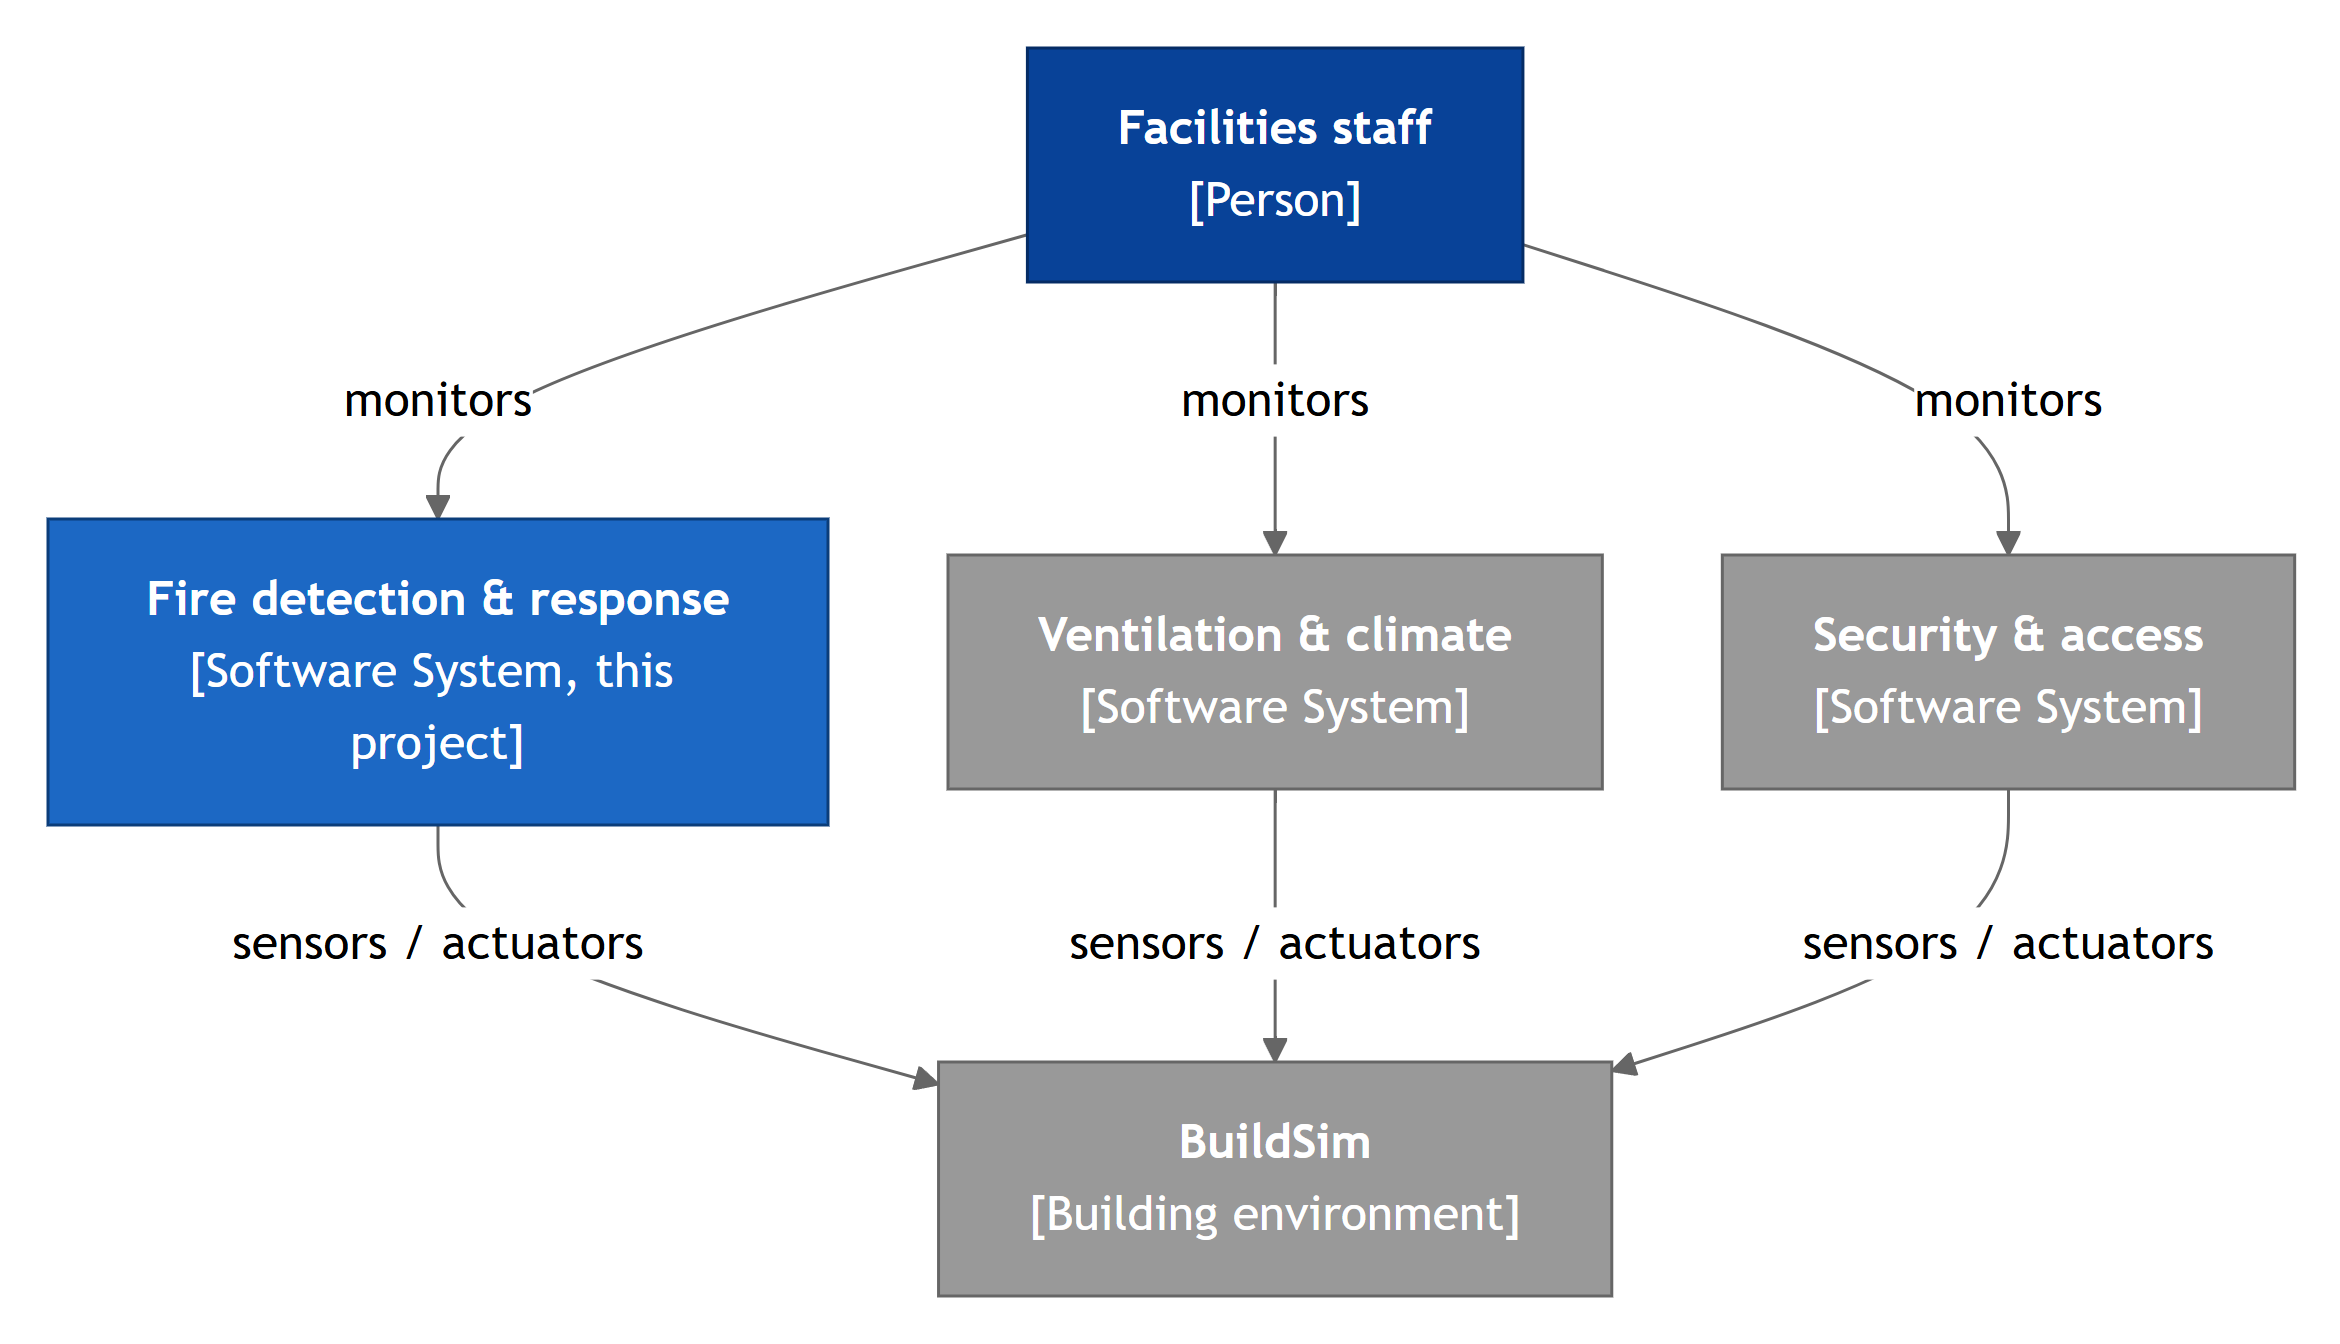
\includegraphics[width=0.85\linewidth]{images/landscape.png}
\caption{C4 System Landscape. Several building systems share one BuildSim; the highlighted one is designed here.}
\label{fig:landscape}
\end{figure}

\section{3. Requirements}\label{sec:requirements}

Every requirement is a testable statement with a stable ID. Functional requirements
(FR) say what the system does, safety requirements (SR) say what it must never do
whatever the agent decides, and non-functional requirements (NFR) say how well. The
last column names the test or experiment that verifies it; the test plan in
Section~10 and the results in Section~11 close the loop.

\begin{longtable}[]{@{}
  >{\raggedright\arraybackslash}p{(\columnwidth - 8\tabcolsep) * \real{0.08}}
  >{\raggedright\arraybackslash}p{(\columnwidth - 8\tabcolsep) * \real{0.28}}
  >{\raggedright\arraybackslash}p{(\columnwidth - 8\tabcolsep) * \real{0.08}}
  >{\raggedright\arraybackslash}p{(\columnwidth - 8\tabcolsep) * \real{0.30}}
  >{\raggedright\arraybackslash}p{(\columnwidth - 8\tabcolsep) * \real{0.26}}@{}}
\toprule
\textbf{ID} & \textbf{Requirement} & \textbf{Priority} & \textbf{Acceptance criterion} & \textbf{Verified by} \\
\midrule
\endhead
FR-01 & Confirm a flaming fire from sensor readings alone & Must & Room reaches \textsc{confirmed} within 180\,s of ignition & \code{test\_agent}, \code{test\_detector}, E1 \\
FR-02 & Confirm a smouldering fire, which has almost no heat & Must & \textsc{confirmed} within 300\,s (the scoreboard's miss limit) & E1 \\
FR-03 & Raise no alarm for cooking, dust, steam, or a drifting sensor & Must & Zero false alarms across all nuisance presets at sensor noise 0--3$\times$ & \code{test\_scoring}, E1, E3 \\
FR-04 & On confirmation: release sprinkler, close the fire door, evacuate & Must & All three commands issued in the confirming tick and journalled with a reason & \code{test\_agent}, E1 \\
FR-05 & Route every evacuee to a real ground-floor exit avoiding alarming rooms & Must & No route crosses an alarming room while a clear one exists; upper floors go down the stairs & \code{test\_evacuation}, \code{test\_walkways}, \code{test\_multifloor} \\
FR-06 & Explain every decision & Must & P(fire) is the sum of named contributions, or the model's verdict with its evidence and a one-line reason; every command and every refusal carries a reason & \code{test\_detector}, \code{test\_llm\_detector}, dashboard \\
FR-07 & Score the run against ground truth & Should & Detections, misses, false alarms, alarm delay and RSET reported live and exportable as CSV & \code{test\_scoring}, \code{test\_history} \\
FR-08 & A second detector behind the same protocol, switchable while running & Should & The language model scores rooms from readings only; the agent, interlocks and panel are unchanged; the panel can switch back & \code{test\_llm\_detector}, \code{test\_layering}, E7 \\
SR-01 & Water needs heat corroboration & Must & A sprinkler request is refused while the room's true temperature is below 35\,°C & \code{test\_interlocks}, E1 \\
SR-02 & Fire doors never lock & Must & A lock command is refused unconditionally & \code{test\_interlocks} \\
SR-03 & Never seal people in & Must & A close command is refused while the room is occupied or on an active escape route & \code{test\_interlocks}, \code{test\_publisher\_doors} \\
NFR-01 & Keep up with the clock & Must & One engine tick over the full building finishes inside the 250\,ms tick budget at 1$\times$; the breaking point at 40$\times$ is measured & E5 \\
NFR-02 & Survive a lying sensor & Must & A stuck, dropping-out or drifting smoke detector does not stop a flaming fire being confirmed & \code{test\_sensing}, E4 \\
NFR-03 & Be repeatable & Must & The same seed gives the same run, tick for tick & \code{test\_reset}, E1 (rerun) \\
NFR-04 & Keep the truth out of the intelligence & Must & No module downstream of the sensors imports or reads the true room state & \code{test\_layering} \\
NFR-05 & Not flood BuildSim & Should & At most 24 sensor writes per publish; the viewer route and highlights are sent only when they change & \code{test\_publishing\_route} \\
NFR-06 & Never wait for the model & Must & A tick never blocks on the network; a room with no fresh verdict is scored by the rule; a malformed answer is refused, not guessed at & \code{test\_llm\_detector} \\
NFR-07 & Never outrun the model & Must & A verdict older than 60 simulated seconds is not used; the speed dial is capped at what measured answer times allow, and the journal says so & \code{test\_pacing}, \code{test\_llm\_detector}, E7 \\
\bottomrule
\end{longtable}

There is a tension in this table. FR-01 and FR-02 want the alarm early;
FR-03 wants it late enough to be sure; SR-01 to SR-03 may refuse the response the
alarm asks for. The dwell times in the state machine resolve the first tension and
the interlocks resolve the second, and the evaluation reports where each of those
compromises costs something. NFR-06 and NFR-07 pull against each other too: a
detector that answers eight seconds late is useless at forty times real time, so
either the clock slows down or the rule takes over, and the system does the first
and falls back to the second. The safety requirements apply whichever detector is
installed; that is the point of keeping the interlocks outside the intelligence.

\textbf{Traceability.} The five architecture viewpoints map onto this document:
context (Section~4.1), functional (4.2 and 4.3), information (Sections~5 to~7),
behavioural (Section~8) and deployment (Section~9). Each requirement names the
design that satisfies it and the test that proves it.

\section{Architecture}\label{sec:architecture}

\subsection{Context diagram (C4 Level 1)}\label{sec:context}

The context view sets the system's boundary. Everything the system knows about the
building comes through BuildSim's REST API. Everything it does to the building goes
back the same way. The operator uses a browser. The occupants are simulated inside
the system. I show them here as the people the system is for, because the safety
rules (interlocks) exist to protect them. There is one piece of outside compute, and
it is optional: the language model endpoint. When that detector is selected, the
service asks it about one room at a time. The other candidate was the overnight
model training from the proposal, and I did not need it. Nothing the system does to
the building depends on the endpoint answering.

\begin{figure}[H]
\centering
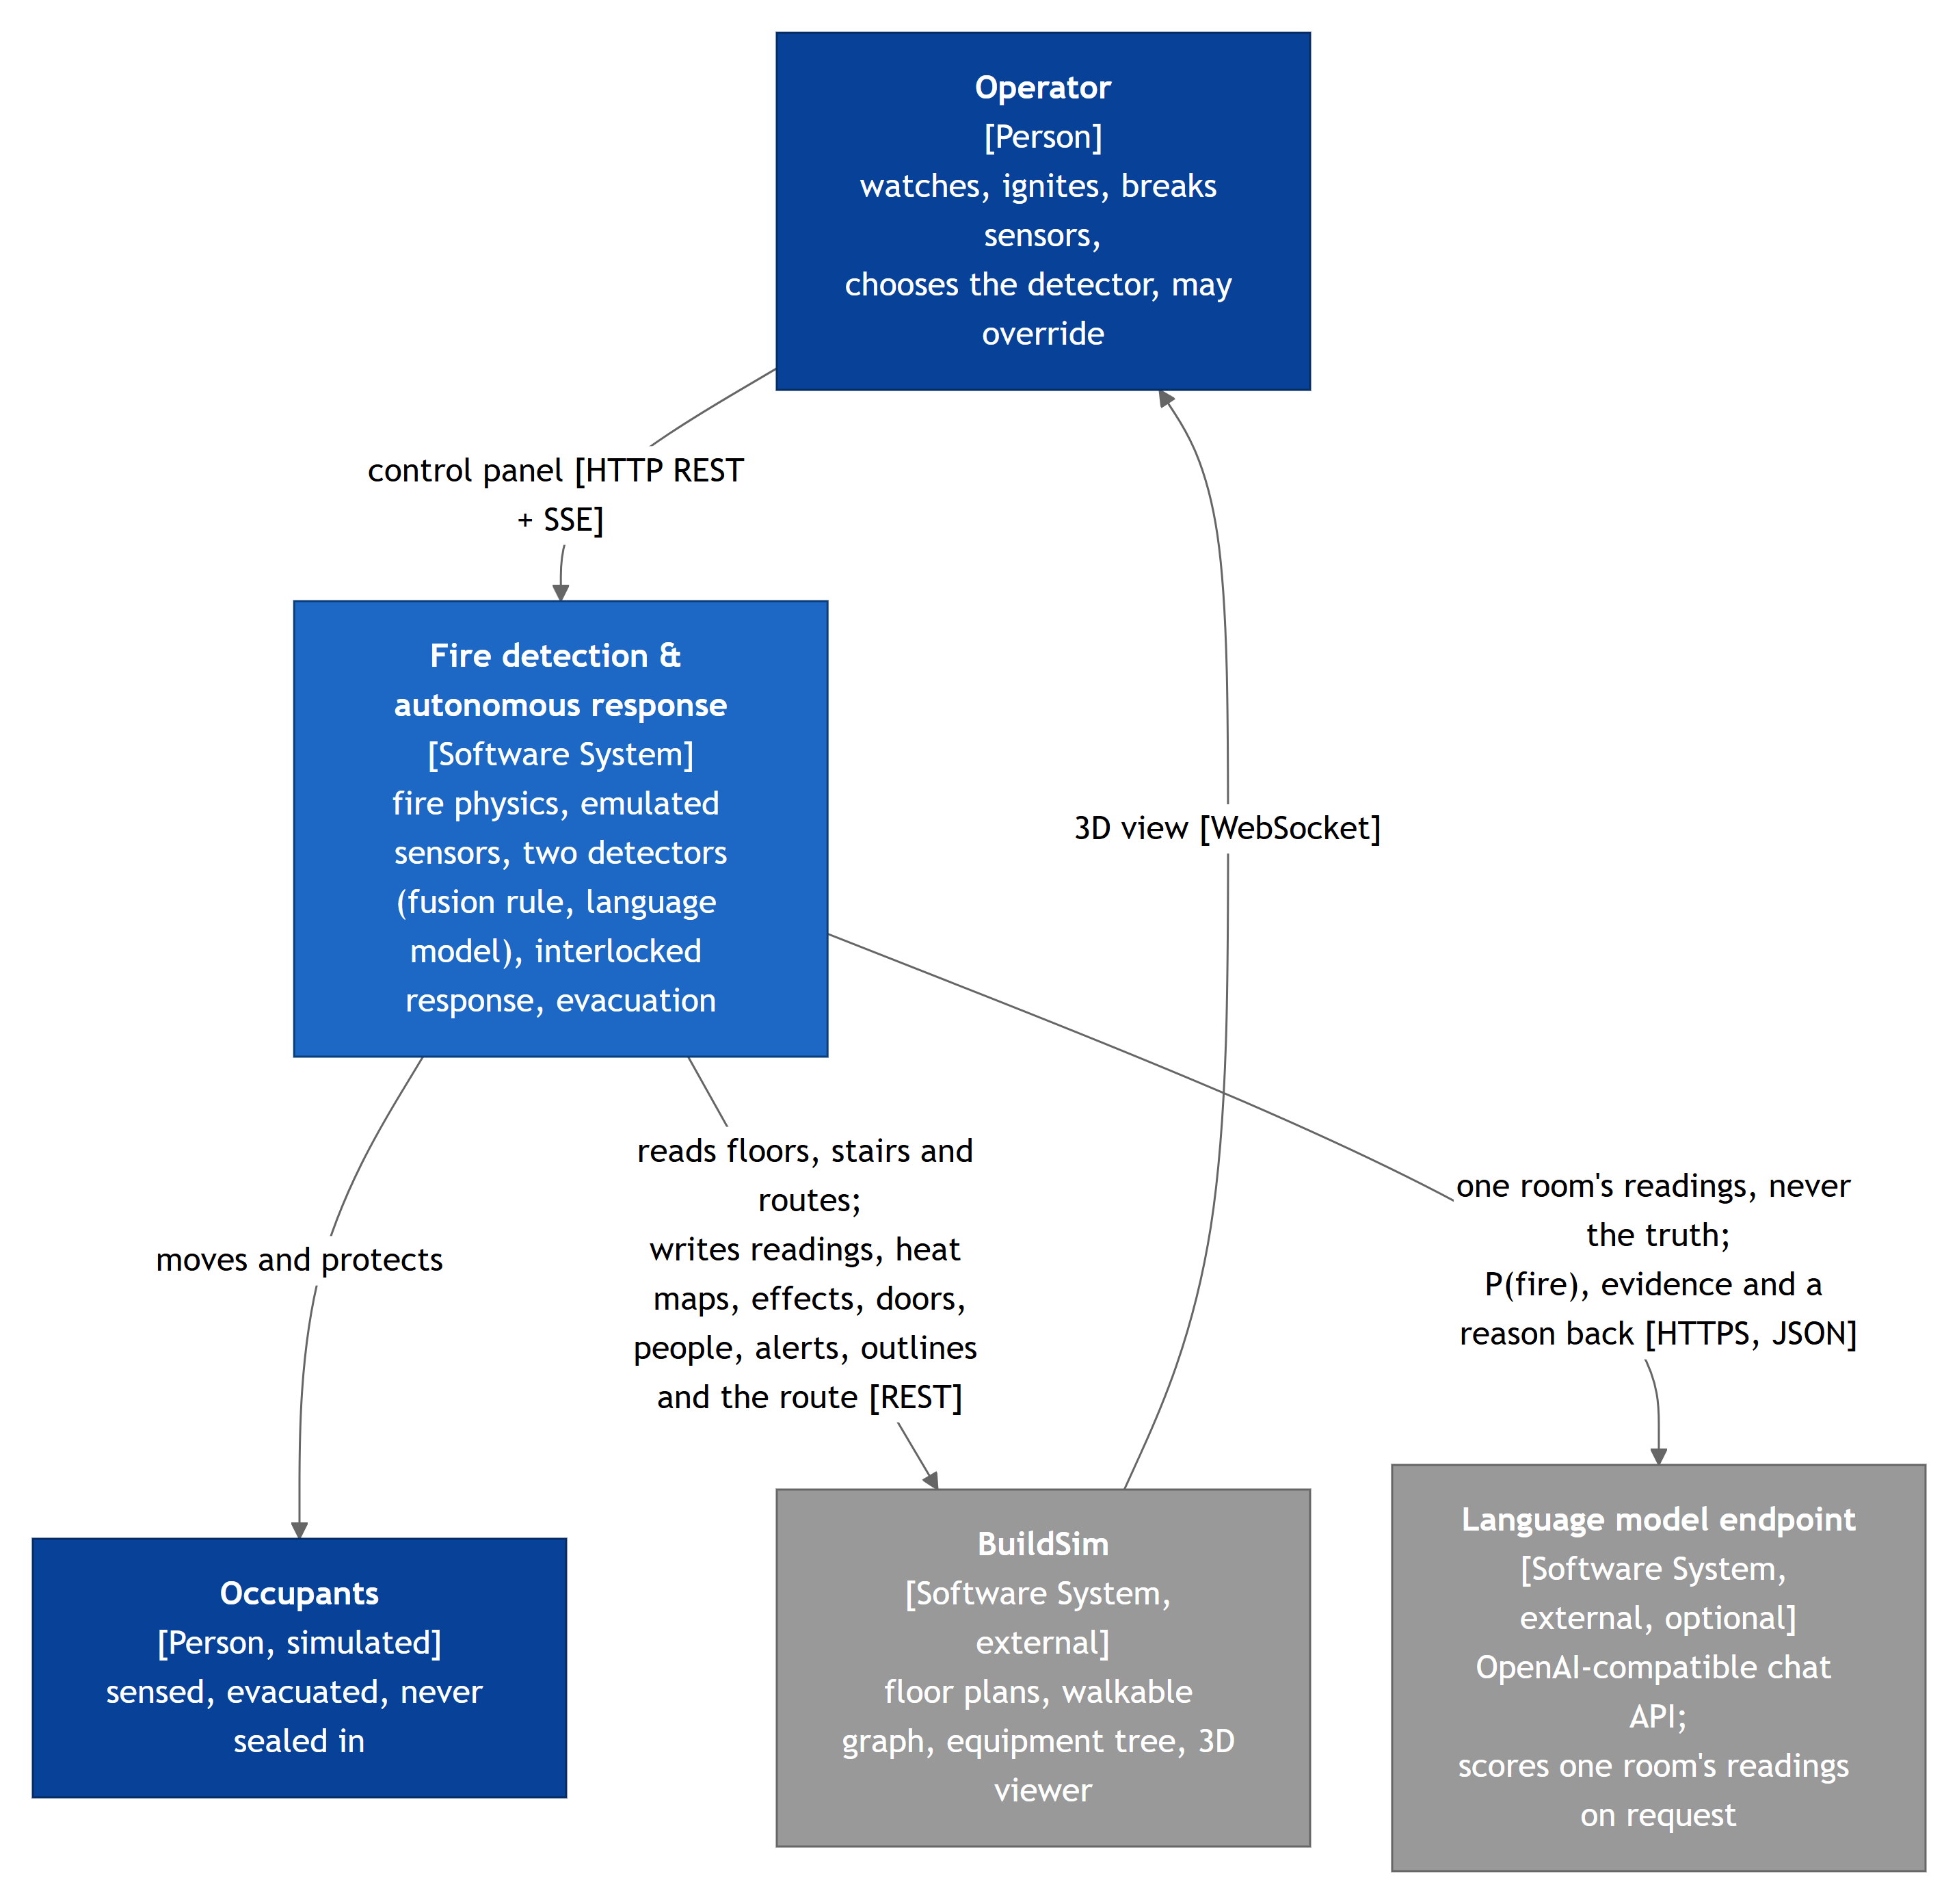
\includegraphics[width=0.78\linewidth]{images/context.png}
\caption{C4 System Context (Level 1). The system in scope is blue. BuildSim (grey) and the language model (purple) are outside it. Every arrow says what it carries. The model only ever gets readings, never the truth.}
\label{fig:context}
\end{figure}

\subsection{Container diagram (C4 Level 2)}\label{sec:container}

The container view opens the box. Five parts run separately, and two of them are my
code: the control panel in the browser and the firelab service. BuildSim and its 3D
viewer are provided. The fifth, the model endpoint, is the only one not on the
laptop. It is also the only one the system runs fine without.

\begin{figure}[H]
\centering
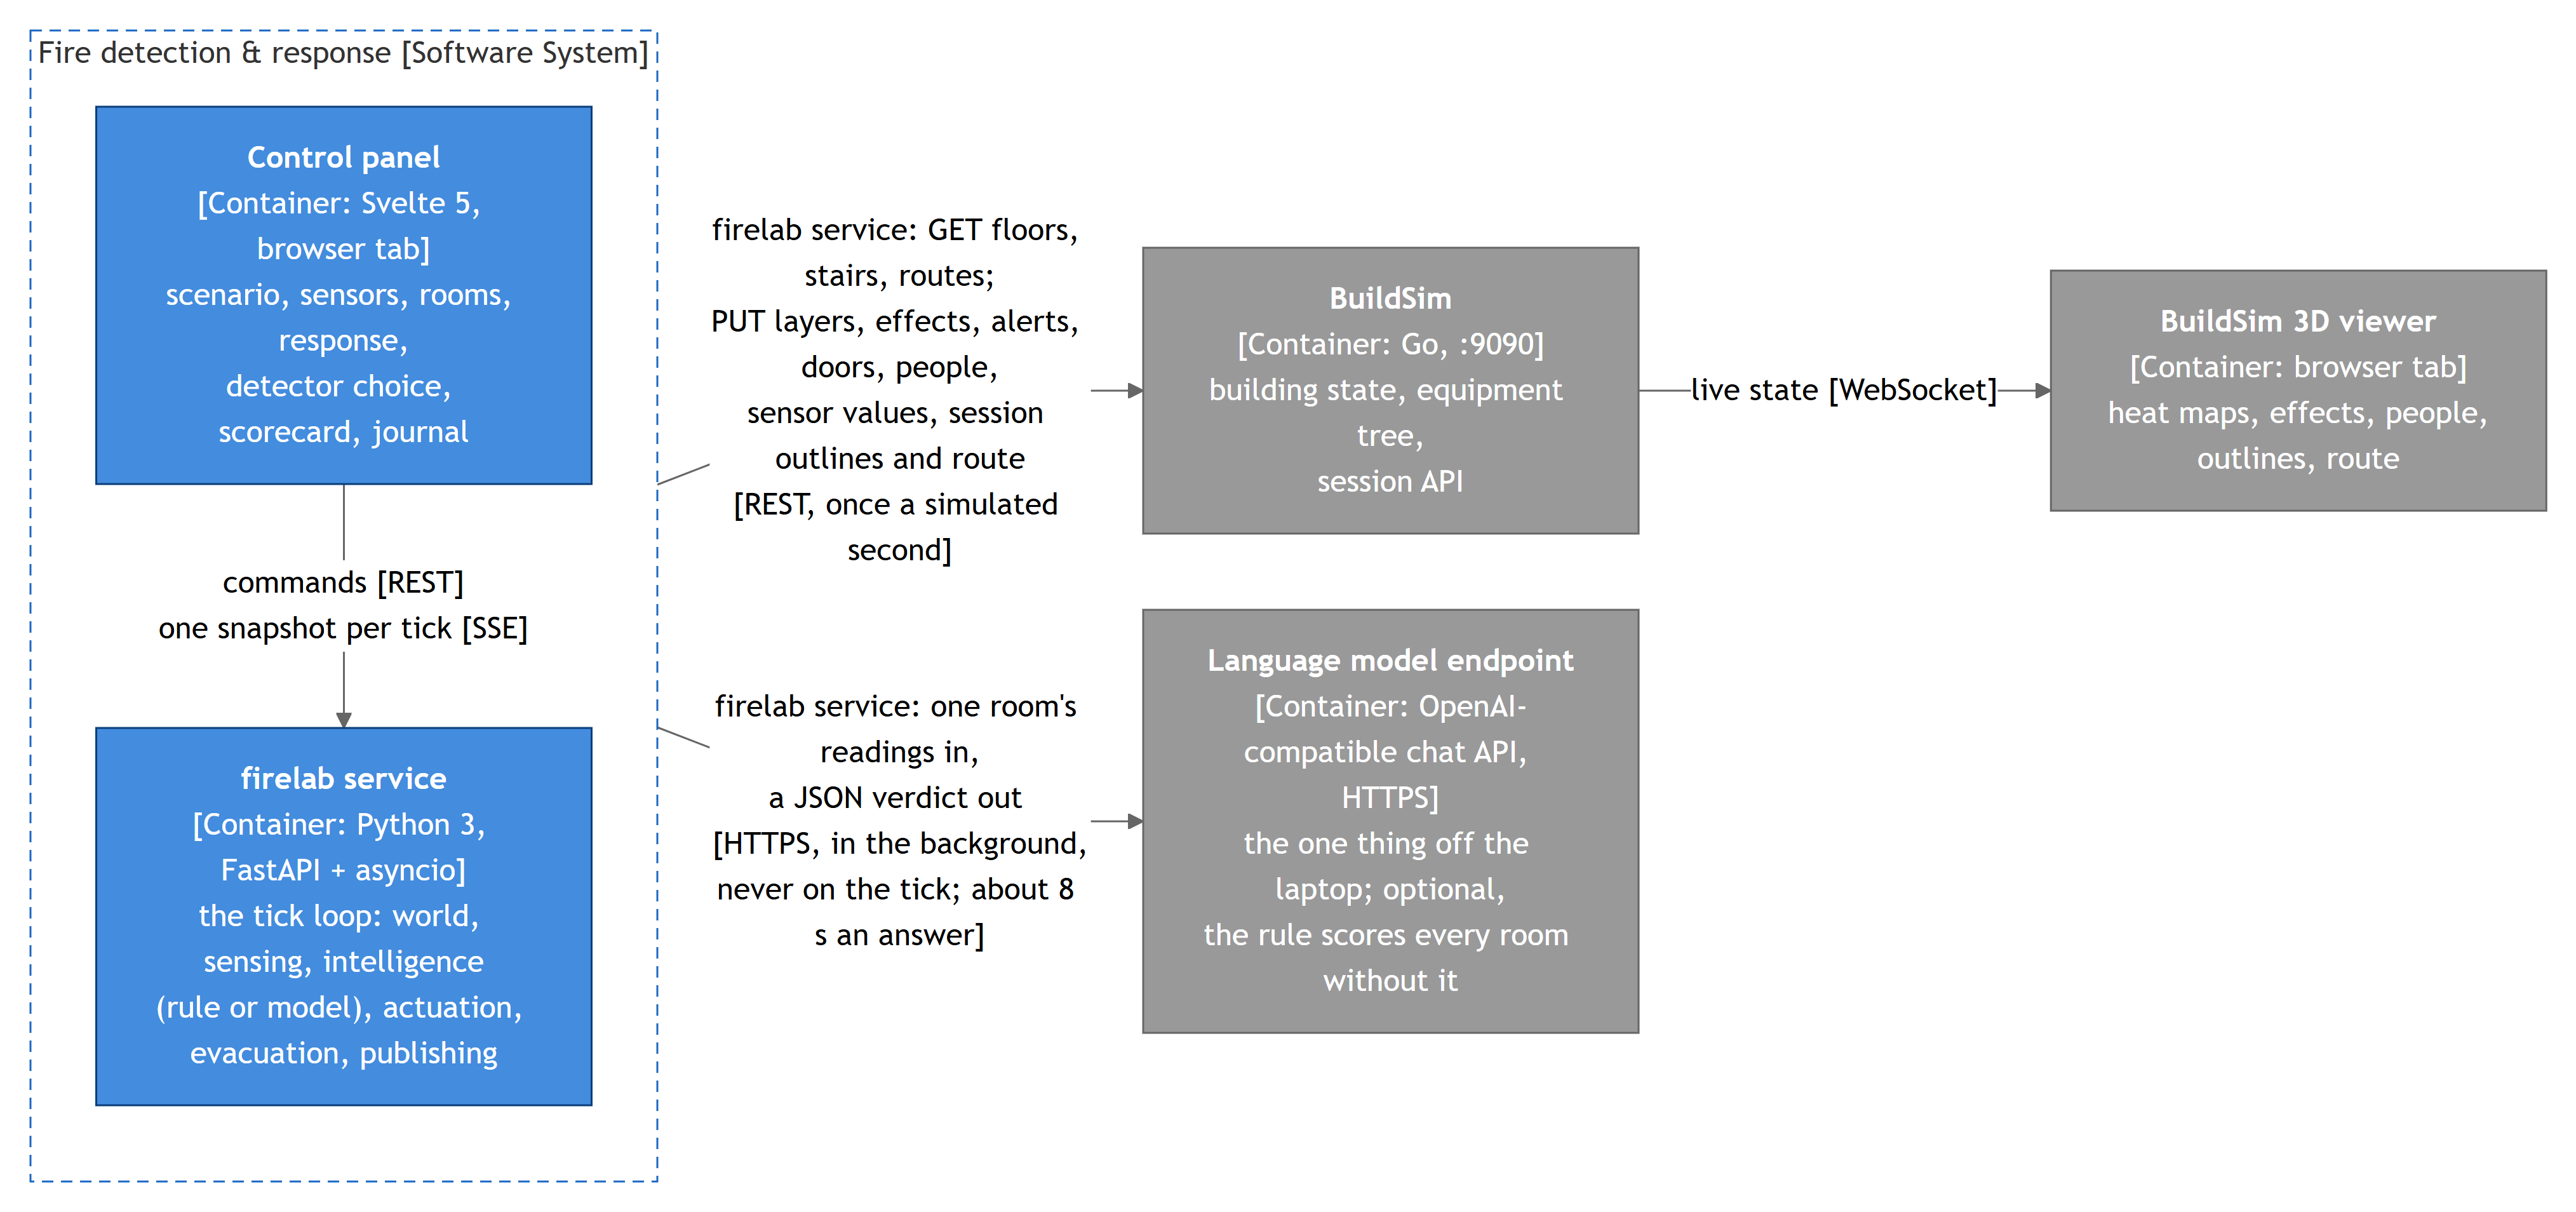
\includegraphics[width=0.90\linewidth]{images/container.png}
\caption{C4 Container diagram (Level 2). The dashed boundary is the system. BuildSim and its viewer are grey, and the language model is purple. Every arrow shows its protocol. A background task calls the model, never the tick.}
\label{fig:container}
\end{figure}

\textbf{Why one service.} In the proposal, nine containers would each have held one
of the four zones. I did not build it that way, for one reason: simulated time. The
whole point of the system is to run a fire at forty times real time. A 25-second
waiting time must still mean 25 simulated seconds. With a broker, every message
would need a simulated timestamp. Every subscriber would have to wait for every
publisher before moving on. A slow dashboard could stall the physics. Inside one
process, the tick loop does four things in a fixed order under one lock. It moves the
world forward, samples the sensors, thinks and acts. ``Now'' is one number. The
price is that the zones share a process, so a crash in one takes down the others.
Section~\ref{sec:risks} says what that costs and what would change if the system left the laptop.

\textbf{How one process does several things at once.} I built the service on
Python's \code{asyncio}. Think of it as one worker that juggles many small jobs.
Whenever a job has to wait, the worker puts it down and picks up another. Most of
the work here is waiting: for BuildSim to reply, for the model to reply, or for a
browser to collect the next update. Four jobs share the worker:
\begin{itemize}[nosep]
  \item the tick, which wakes every 250\,ms and moves the fire forward;
  \item the web API, which answers the control panel and streams live updates to
    each open browser tab;
  \item the publisher, which sends all its updates to BuildSim at once (six fixed
    ones plus one per sensor), so it only waits as long as the slowest one;
  \item the model's helper, which asks the language model its questions in the
    background.
\end{itemize}
I chose one worker instead of several threads because two jobs can then never
change the same data at the same moment. A job can only be paused at a point
where it waits. The tick also holds a lock while it runs, so a button press can
never change the building halfway through a tick. The downside is that a slow job
that never waits holds everyone up. That is why the tick must finish within
250\,ms, and why experiment E5 measures how many rooms fit in that time.

\textbf{What keeps the zones apart} is the package layering, since there are no
process boundaries. There are three packages. \code{domain} is pure: standard library
only, no clock, no network. \code{adapters} holds everything that speaks HTTP to
BuildSim. \code{app} holds the tick loop, the API and the snapshot. Dependencies only
point inward. A test, \code{test\_layering}, fails the build if any module imports
the wrong way. It also fails if anything in the intelligence path touches the true
room state.

\textbf{The control panel} is a separate container because it has a different
lifecycle. I build it once with Vite into static files, and the service serves them.
It talks to the service only through the REST endpoints and the server-sent event
stream. A script would use the same interface. The panel knows nothing about the
engine's internals.

\textbf{The model endpoint} is outside the boundary for the opposite reason. It is
not mine, and other users share it. It answers in about eight real seconds, while
the tick has 250 milliseconds. Those two facts shaped the adapter in front of it.
The service never waits for the model and asks it about one room at a time. It uses
an answer for at most a minute of simulated time. It also slows the clock to what the
measured answer time allows, so answers do not go stale (Section~\ref{sec:service}). I chose an
OpenAI-compatible chat API because every hosted and local model server speaks it.
So the endpoint, the key and the model name are three environment variables, and
nothing in the code names a vendor.

\subsection{Component diagram (C4 Level 3): inside the firelab service}\label{sec:component}

The service is the one container complex enough to need its own picture. Its
components are the four zones of one tick, plus the parts around them. The three
groups mark the truth boundary. Components in the orange group may read the real
state of the rooms. Components in the two blue groups may not. The only thing that
leaves the orange group is a sensor reading. I put the LLM adapter in the
readings-only group on purpose. It speaks HTTPS, so by the layering rules it lives
under \code{adapters}. But it sends the same feature vector the rule sees. The
layering test checks that it imports nothing that could tell it the truth.

\begin{figure}[H]
\centering
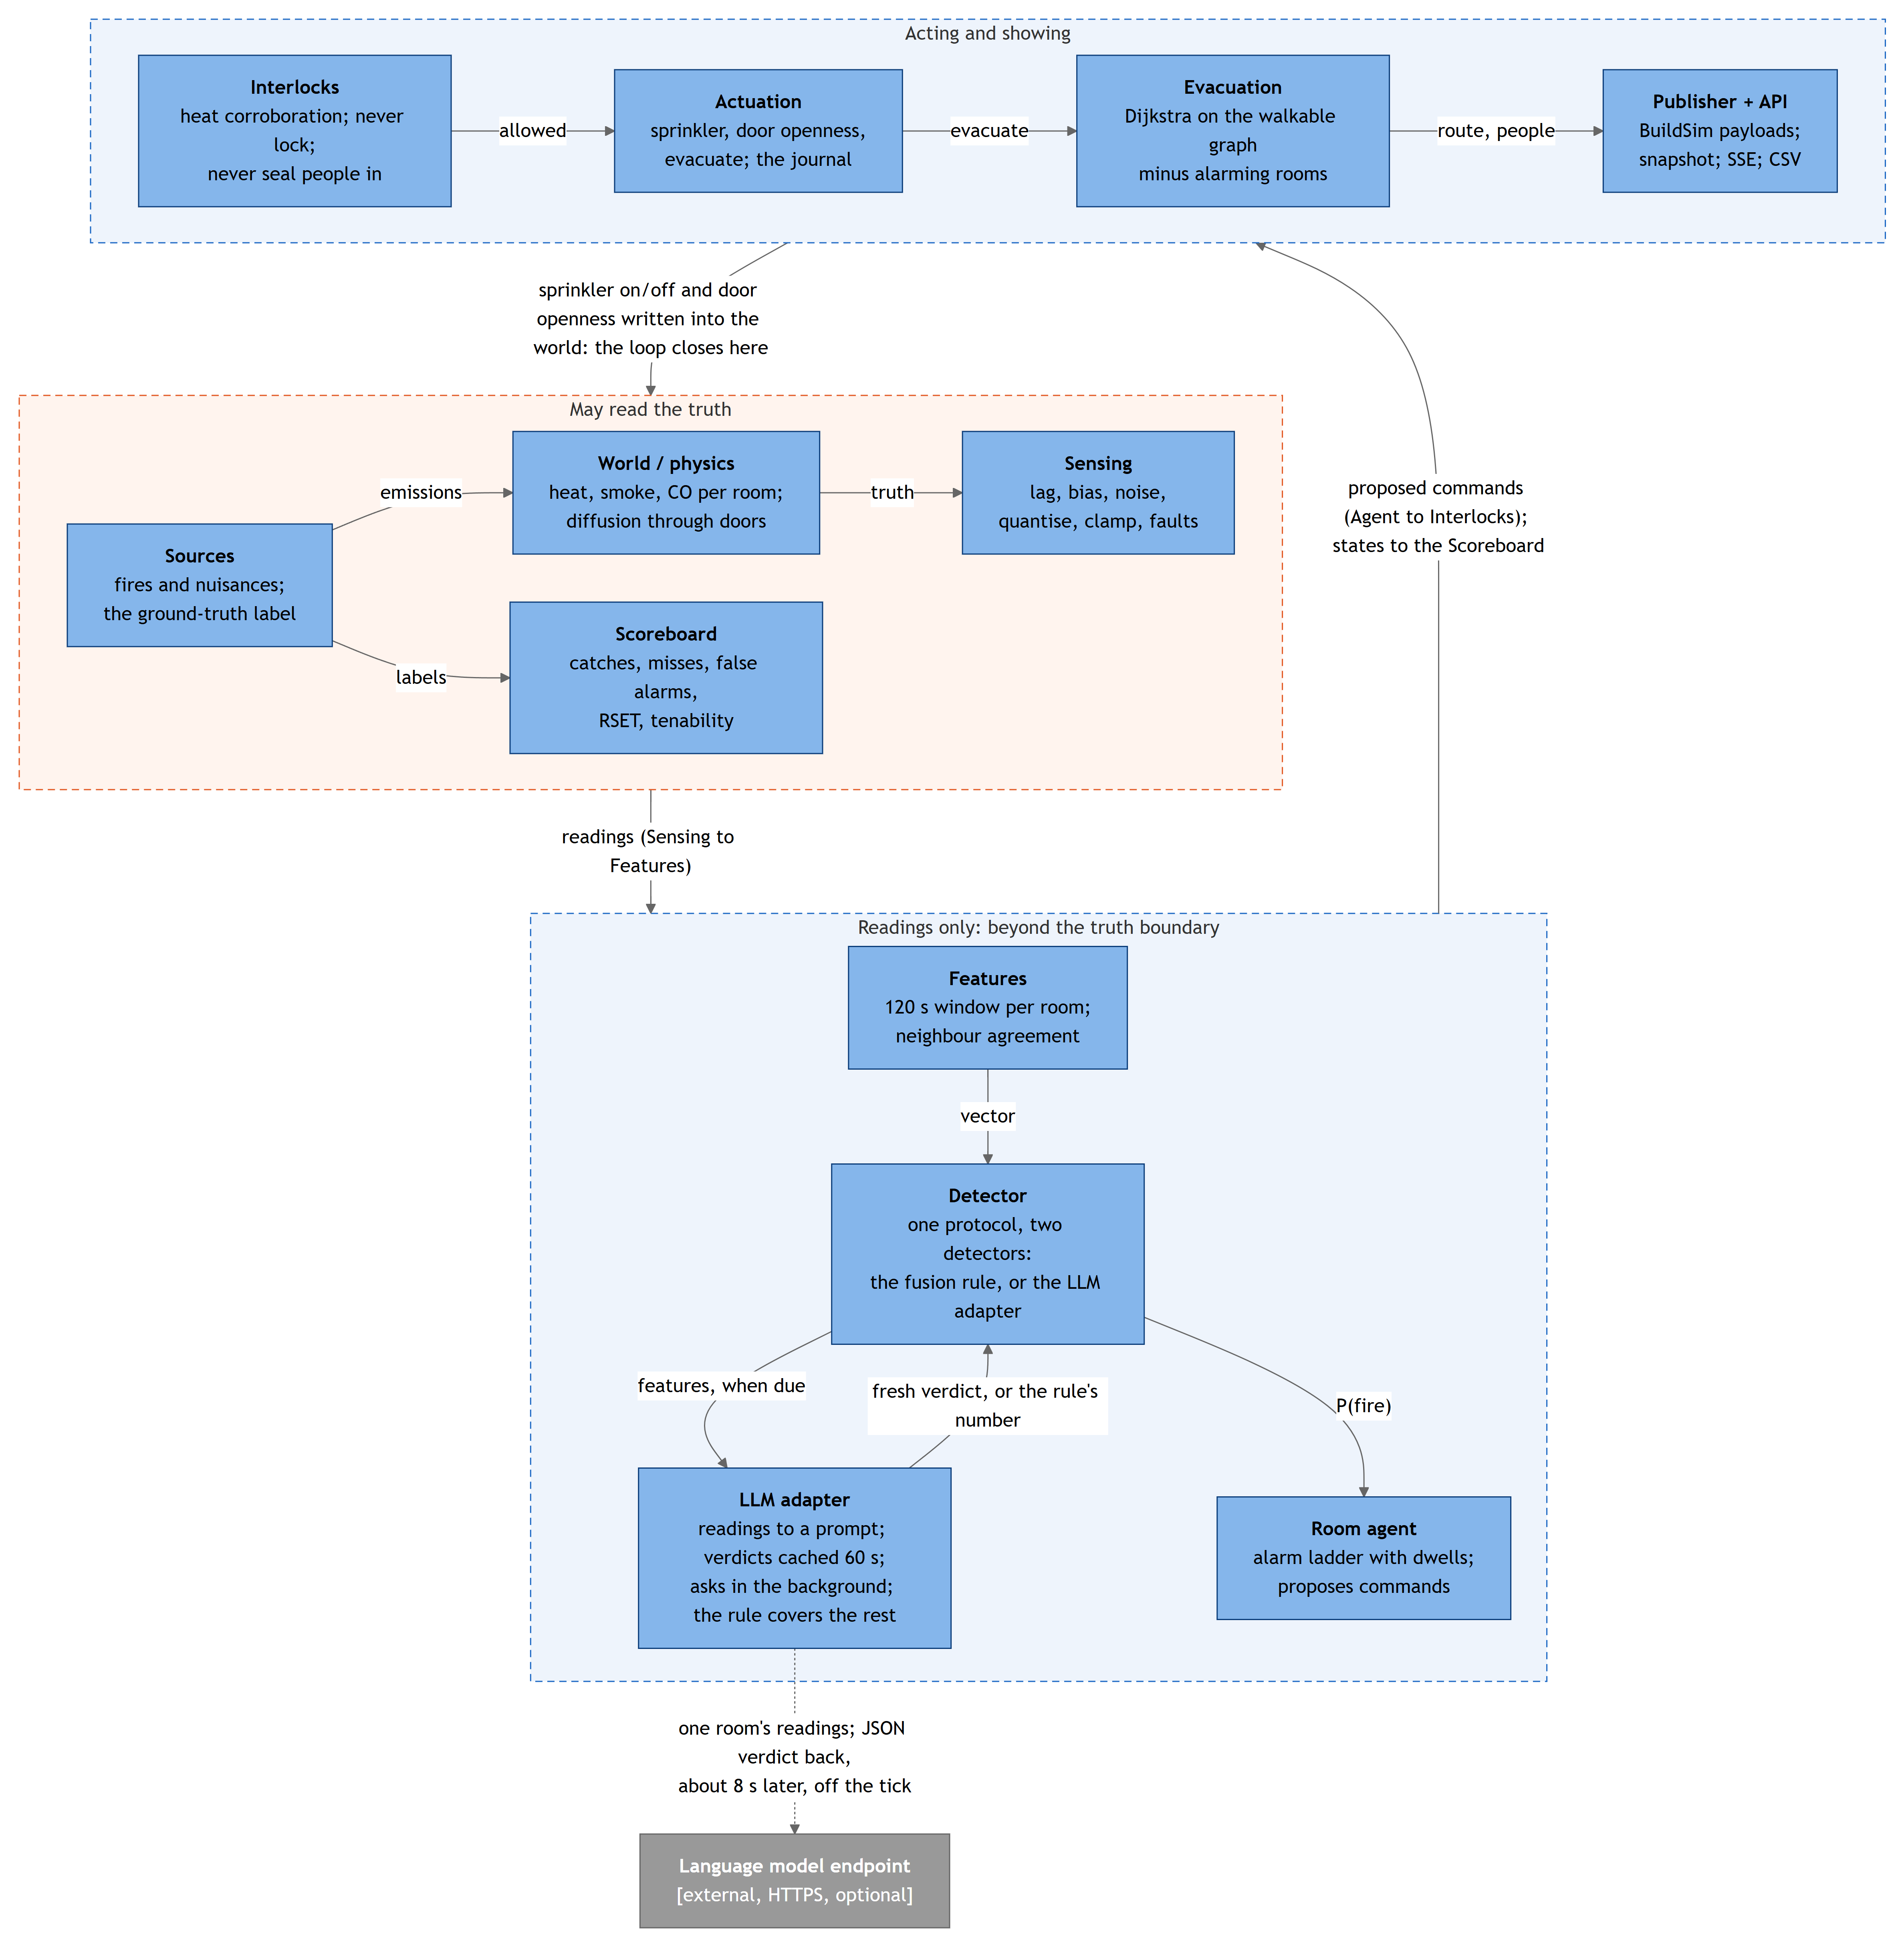
\includegraphics[width=1.00\linewidth]{images/component.png}
\caption{C4 Component diagram (Level 3) of the firelab service. The groups run in this order every tick: the orange group (the world and the sensors), then the green group (the detector and the agent), then the blue group (the actions). Only readings leave the orange group, and the layering test fails if anything else does. The thick line from the blue group back to the orange one is the sprinkler and door state being written into the world. The dotted arrow is the one call that leaves the process: the LLM adapter asking the language model about a room, outside the tick.}
\label{fig:component}
\end{figure}

\textbf{Component responsibilities.} Each component has one job. The last column
says why it is a separate component.

\begin{longtable}[]{@{}
  >{\raggedright\arraybackslash}p{(\columnwidth - 6\tabcolsep) * \real{0.15}}
  !{\colsep}>{\raggedright\arraybackslash}p{(\columnwidth - 6\tabcolsep) * \real{0.31}}
  !{\colsep}>{\raggedright\arraybackslash}p{(\columnwidth - 6\tabcolsep) * \real{0.24}}
  !{\colsep}>{\raggedright\arraybackslash}p{(\columnwidth - 6\tabcolsep) * \real{0.30}}@{}}
\toprule
\rowcolor{tablehead}
\textbf{Component} & \textbf{Responsibility (one job)} & \textbf{Module} & \textbf{Reason for separation} \\
\midrule
\endhead
Sources & What a fire, or cooking, dust or steam, gives off over time. Carries the ground-truth label & \code{domain/sources.py} & The label must never leak: only the scoreboard reads \code{kind} \\
\rowline
World / physics & One lumped node per room. Each node settles towards the level its sources drive it to, and spreads through doors and stairs & \code{domain/physics.py} & Owns every time constant, so each source stays a few lines long \\
\rowline
Sensing & Turns the truth into a reading through the corruption chain. Holds faults & \code{domain/sensing.py} & The line between truth and what is observed. The one place noise and faults live \\
\rowline
Features & A 120\,s window per room: rate of rise, ratio, neighbour agreement & \code{domain/features.py} & Sees readings only. This is the detector's input contract \\
\rowline
Detector & Turns features into P(fire), the estimated chance that the room is on fire, with a contribution per feature. The fusion rule (my hand-written rule that combines the sensor features into one score) is one implementation & \code{domain/detector.py} & A protocol, so a second detector can replace the rule without touching the agent. One did \\
\rowline
LLM adapter & The same protocol, answered from a cache of the model's answers. Asks in the background. The rule covers any room without a fresh answer & \code{adapters/llm/} & The network must never hold up the tick. One file per job (prompt, verdict, policy, client, detector), so each can be tested without an endpoint \\
\rowline
Room agent & The alarm ladder with waiting times. Proposes commands with reasons & \code{domain/agent.py} & Decides but never acts. Testable with no actuators \\
\rowline
Interlocks & Allows or refuses a command and says why & \code{domain/interlocks.py} & Kept outside the agent, so even a badly trained agent cannot trap anyone \\
\rowline
Actuation & The only door between deciding and doing. Writes sprinkler and door state into the world & \code{app/engine/actuation.py} & Closes the loop. One audit point for every change \\
\rowline
Evacuation & Routes people around danger, walks them, and picks the one route to draw & \code{app/evacuation.py}, \code{adapters/walkways.py} & The one domain-level job that needs a route lookup \\
\rowline
Scoreboard & Detections, misses, false alarms, RSET (the time people need to get out safely) and tenability (whether a room is still survivable) & \code{domain/scoring.py}, \code{timeline.py}, \code{tenability.py} & Grades the run. The only reader of the truth on the right-hand side \\
\rowline
Publisher + API & Turns engine state into BuildSim payloads and the UI snapshot. REST, SSE, CSV & \code{adapters/publisher/}, \code{app/api/}, \code{app/snapshot/} & Keeps presentation out of the loop. BuildSim's payload shapes live in one place \\
\bottomrule
\end{longtable}

\subsection{Design decisions and justifications}\label{sec:decisions}

Each row names the option I took, the alternative I considered, the requirement it
serves and the price paid. A decision with no rejected alternative would only be an
assumption.

\begin{longtable}[]{@{}
  >{\raggedright\arraybackslash}p{(\columnwidth - 8\tabcolsep) * \real{0.14}}
  !{\colsep}>{\raggedright\arraybackslash}p{(\columnwidth - 8\tabcolsep) * \real{0.20}}
  !{\colsep}>{\raggedright\arraybackslash}p{(\columnwidth - 8\tabcolsep) * \real{0.18}}
  !{\colsep}>{\raggedright\arraybackslash}p{(\columnwidth - 8\tabcolsep) * \real{0.30}}
  !{\colsep}>{\raggedright\arraybackslash}p{(\columnwidth - 8\tabcolsep) * \real{0.18}}@{}}
\toprule
\rowcolor{tablehead}
\textbf{Decision} & \textbf{Chosen} & \textbf{Alternatives} & \textbf{Justification (requirement)} & \textbf{Trade-off} \\
\midrule
\endhead
Process model & One tick loop, four zones, one lock & One container per zone over MQTT (the proposal) & Waiting times and rates need one simulated clock. At 40$\times$, a reading sent through a broker is stale when it arrives (NFR-01, NFR-03) & No fault isolation between zones. Splitting them is a future step \\
\rowline
Concurrency & \code{asyncio}: one worker that switches between jobs while they wait & Several threads; one process per job & The work is mostly waiting on the network. With one worker, two jobs never change the same data at once, and the tick's lock covers the rest (NFR-01, NFR-03) & A slow job that never waits holds everyone up, so the tick must finish within 250\,ms \\
\rowline
Zone separation & Import layering checked by a test & Trust the code review & The truth is one attribute away from the detector. A test lets me check that the code keeps away from it (NFR-04) & A test to maintain as modules move \\
\rowline
Detector & Hand-written fusion rule behind a protocol, as the default & Isolation forest; autoencoder; the model alone & It caught every fire, with zero false alarms at every noise level. It explains itself term by term and costs nothing per room (FR-01, FR-03, FR-06) & Weights tuned by hand. No learning from data \\
\rowline
Second detector & A language model over an OpenAI-compatible API, given readings only & Isolation forest trained on exported runs; no second detector & This is the comparison the proposal promised, without training on the simulator's own output. The answer comes with evidence and a reason, so FR-06 still holds (FR-08) & About 8\,s per answer, not repeatable, and an outside dependency \\
\rowline
Model off the tick & Background worker, cached answers good for 60\,s, rule fallback & Ask and wait for the reply; use stale answers & A tick has 250\,ms and an answer takes seconds. A room must always have a number, and a stale number is a wrong one (NFR-06, NFR-07) & Two detectors are in play at once, and the journal has to say which one is speaking \\
\rowline
Pacing & Cap the speed dial at what measured answer times allow & Let the clock run and accept that answers expire & At 40$\times$, every answer arrived 320 simulated seconds late, and the rule quietly did all the work. A capped dial is honest (NFR-07) & With this endpoint, the demo runs at 3$\times$ instead of 40$\times$ \\
\rowline
Questions in flight & One at a time, most suspicious room first & Several at once & The endpoint answers requests one after another. Two in flight doubled the delay and halved the speed the clock could run at. The fire room gets its answer first & The rule scores most of the quiet neighbours \\
\rowline
Alarm logic & State machine with waiting times & Threshold on P(fire) & A single threshold flickers with noise. Waiting times cost seconds, but they stop doors opening and closing over and over (FR-03) & Adds 45\,s to confirming a clear fire \\
\rowline
Safety & Safety rules outside the agent & Rules inside the agent's policy & Whoever is wrong upstream, the building stays safe. The same check applies to a person's click (SR-01 to SR-03) & A confirmed fire in an occupied room gets no door \\
\rowline
Deferred commands & A refused request stands until it can be carried out & Refuse once and forget & ``Not yet'' must not become ``never''. In the smoulder, the sprinkler was refused at 201\,s and released at 219\,s, once heat arrived (SR-01) & Re-checked every tick \\
\rowline
Route search & My own Dijkstra search over BuildSim's graph, with alarming rooms removed & Ask BuildSim's router for each exit & BuildSim only returns the shortest path. A fire in a corridor makes every shortest path run through it (FR-05) & A second copy of the graph to keep consistent \\
\rowline
Sensor emulation & Lag, bias, noise, quantisation, clamp, faults per device & Truth plus Gaussian noise & The interesting failures (saturation, stuck, dead) are not noise. The temperature clamp at 250\,°C is what a real heat detector does (NFR-02) & More parameters to defend \\
\rowline
Physics & Lumped node per room, first-order relaxation, door-gated diffusion & CFD; zone model with layers & Enough structure to close the loop and get the trends right. Cheap enough for 956 rooms 40 times a second (NFR-01) & The fire room overheats when sealed. No oxygen limit (Section~\ref{sec:risks}) \\
\rowline
Storage & In-memory rolling windows; CSV export & Time-series database; ThingsBoard & The detector may only see 120\,s, and the charts only need 20 minutes. A database would be one more process to keep in step with the clock (NFR-01) & History is lost on restart. Long runs are exported, not stored \\
\rowline
UI transport & Server-sent events, one snapshot per tick & Polling; WebSocket & One-way push with automatic reconnect, and a plain HTTP stream any tool can read & The snapshot is rebuilt every tick, even with no listener \\
\rowline
BuildSim writes & Once per simulated second, complete collections, 24 sensor values per publish & Every tick; deltas & BuildSim replaces a whole collection on each write. Too many writes overloaded it (NFR-05) & Sensor labels in the tree lag behind the truth \\
\bottomrule
\end{longtable}

\section{Interfaces and communication}\label{sec:interfaces}

I use four patterns, each where it fits. \textbf{REST} carries every command and
every call to BuildSim. Each is a one-to-one request, and the caller must know the
result. For example, a refused command comes back with the safety rule's reason.
\textbf{Server-sent events} carry the snapshot to the control panel. That flow is
one-way and high-rate, and it needs no reply. \textbf{WebSocket} is BuildSim's own
channel to its viewer. I use it, but I did not build it. \textbf{HTTPS chat
completions} carry one room's readings to the language model and a JSON answer back.
A background task makes the call, with a 30\,s timeout and one retry. The result
goes into a cache, never into a tick. There is no pub/sub, for the reason given in
Section~\ref{sec:container}.

\textbf{Naming.} Everywhere, a room's address is \code{level/name}, for instance
\code{level2/A3505}. I do this because a bare name is not unique across storeys. A
device is \code{fl-<level>-<room>-<modality>}, so you can read its room and sensor
type off its ID. Units are fixed and never sent in messages: temperature in °C,
smoke as optical obscuration in 1/m, CO in ppm, distances on the plan in half-metre
units, and simulated time in seconds since midnight.

\textbf{The control-panel API.} Every request body is a typed model. The framework
rejects unknown keys before the engine sees them.

\begin{longtable}[]{@{}
  >{\raggedright\arraybackslash}p{(\columnwidth - 6\tabcolsep) * \real{0.10}}
  !{\colsep}>{\raggedright\arraybackslash}p{(\columnwidth - 6\tabcolsep) * \real{0.30}}
  !{\colsep}>{\raggedright\arraybackslash}p{(\columnwidth - 6\tabcolsep) * \real{0.30}}
  !{\colsep}>{\raggedright\arraybackslash}p{(\columnwidth - 6\tabcolsep) * \real{0.30}}@{}}
\toprule
\rowcolor{tablehead}
\textbf{Method} & \textbf{Path} & \textbf{Body} & \textbf{Semantics} \\
\midrule
\endhead
GET & \code{/api/state} & & The full snapshot, once \\
\rowline
GET & \code{/api/events} & & SSE: one snapshot per tick, 4\,Hz \\
\rowline
GET & \code{/api/rooms} & & Every space for the pickers \\
\rowline
GET, PUT & \code{/api/config} & partial config & Live settings: speed, thresholds, waiting times, noise, population. \code{detector.kind} swaps the detector on the next tick \\
\rowline
POST & \code{/api/clock} & \code{\{seconds?, factor?, running?\}} & Play, pause, jump, 0.1--600$\times$ \\
\rowline
POST & \code{/api/scenario/ignite} & \code{\{space, kind, growth, delay, peak\_kw\}} & Schedule a source. \code{kind} is also the label \\
\rowline
POST & \code{/api/scenario/preset} & \code{\{preset, space\}} & Put sensors in the room and its neighbours, then ignite \\
\rowline
DELETE & \code{/api/scenario/\{id\}} & & Put a source out. What it gave off still spreads \\
\rowline
POST & \code{/api/sensors/deploy} & \code{\{spaces, modalities\}} & Install devices. A room without devices is not monitored \\
\rowline
POST & \code{/api/sensors/fault} & \code{\{device\_id, fault\}} & \code{stuck | dropout | drift | dead | none} \\
\rowline
POST & \code{/api/agent/mode} & \code{\{auto\}} & \code{false} means supervised: decisions are shown, not carried out \\
\rowline
POST & \code{/api/actuators/command} & \code{\{kind, space, value\}} & A manual command. It passes the same safety rules and returns \code{\{allowed, reason\}} \\
\rowline
GET & \code{/api/history?space=} & & The last 240 samples of one room \\
\rowline
GET & \code{/api/export.csv} & & Truth beside reading beside P(fire), every room, labelled \\
\rowline
POST & \code{/api/reset}, \code{/api/reload} & & Quiet building. Reload floors from BuildSim \\
\bottomrule
\end{longtable}

\textbf{The snapshot} is the one data structure the panel reads. Each monitored room
appears as shown below. The three columns of the Rooms table are the three objects
in it: what is true, what was reported, and what the system believes.

\begin{verbatim}
{"key": "level2/A3505", "level": "level2", "name": "A3505", "kind": "room",
 "truth":   {"temperature": 648.0, "smoke": 0.668, "co": 107.0},
 "reading": {"temperature": 250.0, "smoke": 0.665, "co": 101.0},
 "p_fire": 0.994, "state": "CONFIRMED", "tenable": false,
 "sprinkler": true, "door": "closed", "occupants": 0,
 "devices": [{"id": "fl-level2-A3505-smoke", "modality": "smoke",
              "fault": "none", "reading": 0.665}, ...]}
\end{verbatim}

The temperature reading of 250 against a truth of 648 is not a bug in the example.
It is the heat detector's range clamp. The snapshot exists to make this kind of
thing visible.

\textbf{The BuildSim interface.} I publish truth and belief to different endpoints.
So a false positive shows on screen as a room glowing red on the belief layer while
it is cool on the heat map.

\begin{longtable}[]{@{}
  >{\raggedright\arraybackslash}p{(\columnwidth - 6\tabcolsep) * \real{0.36}}
  !{\colsep}>{\raggedright\arraybackslash}p{(\columnwidth - 6\tabcolsep) * \real{0.10}}
  !{\colsep}>{\raggedright\arraybackslash}p{(\columnwidth - 6\tabcolsep) * \real{0.32}}
  !{\colsep}>{\raggedright\arraybackslash}p{(\columnwidth - 6\tabcolsep) * \real{0.22}}@{}}
\toprule
\rowcolor{tablehead}
\textbf{Endpoint} & \textbf{Direction} & \textbf{Carries} & \textbf{When} \\
\midrule
\endhead
\code{GET /api/building/floors/\{level\}} & read & rooms, polygons, walkable graph & once, at load \\
\rowline
\code{GET /api/building/cross-floor-edges} & read & stairs and lifts joining storeys & once, at load \\
\rowline
\code{GET /api/graph/route} & read & a shortest path, multi-floor & fallback when no clear route exists \\
\rowline
\code{PUT /api/room-layers} & write & true temperature, smoke, CO; and P(fire) as its own layer & every simulated second \\
\rowline
\code{PUT /api/effects} & write & fire, smoke and sprinkler particles & every simulated second \\
\rowline
\code{PUT /api/alerts} & write & the agent's alarm markers with P(fire) & every simulated second \\
\rowline
\code{PUT /api/doors} & write & fire-door state. Also blocks the walkable router & every simulated second \\
\rowline
\code{PUT /api/entities}, \code{/api/occupancy} & write & every occupant's position and figure; head count per room & every simulated second \\
\rowline
\code{PUT /api/sensors/\{id\}/value} & write & one device's latest reading, into the equipment tree & 24 per publish, round robin \\
\rowline
\code{PUT /api/sessions/\{id\}/highlights} & write & red, orange, yellow outlines by alarm state & when they change \\
\rowline
\code{PUT /api/sessions/\{id\}/route} & write & the one escape route drawn, each node with its storey & when it changes \\
\bottomrule
\end{longtable}

A route is a list of waypoints plus its length in metres. Each waypoint carries its
level, so a path down the stairs is drawn on each storey it crosses. A closed door
goes to BuildSim as well as into the physics. That way BuildSim's own router, which
the viewer's route finder uses, stops sending people into a sealed room.

\textbf{The model interface.} There is one request per room:
\code{POST /chat/completions} on whatever base URL is configured. It holds the fixed
system prompt and the room's readings as plain lines with units. The prompt is the
whole contract. It tells the model that it sees only the sensors, never the room. It
also lists what separates a fire from cooking, dust or steam, in the same terms the
rule uses. The reply must be one JSON object:

\begin{verbatim}
{"p_fire": 0.92,
 "evidence": [{"name": "CO 95 ppm", "weight": 0.30},
              {"name": "smoke rising", "weight": 0.25}, ...],
 "reason": "Smoke, CO and temperature are rising together."}
\end{verbatim}

The service refuses any reply that does not parse as that, or whose probability is
not a number. It does not try to repair it, and the room stays with the rule. The
evidence becomes the ``Why'' bars on the panel. Next to them is a bar for the answer
itself, on the rule's logit scale. That way the two detectors read the same way on
screen.

\section{6. Simulating the sensor values (the physical model)}

BuildSim provides the rooms but nothing that changes, so the fire, the air in every
room, the sensors and the people are all simulated here. The aim was never physical
fidelity. It was a model with enough structure that a decision made on its readings
means something: fires that keep growing, nuisances that peak and fade, smoke that
leaves through doors and climbs stairwells, and, above all, actuator commands that
change the next reading so that the loop closes.

\textbf{Sources.} A source is a scripted event with a kind, a room and a start
time. The kind is also the ground-truth label the scoreboard uses, and nothing
downstream of the sensors may read it. Each kind declares what it emits at time $e$
since ignition, as a heat release rate and the smoke and CO the room would settle
to if nothing else happened:

\begin{longtable}[]{@{}
  >{\raggedright\arraybackslash}p{(\columnwidth - 6\tabcolsep) * \real{0.16}}
  >{\raggedright\arraybackslash}p{(\columnwidth - 6\tabcolsep) * \real{0.16}}
  >{\raggedright\arraybackslash}p{(\columnwidth - 6\tabcolsep) * \real{0.34}}
  >{\raggedright\arraybackslash}p{(\columnwidth - 6\tabcolsep) * \real{0.34}}@{}}
\toprule
\textbf{Kind} & \textbf{Label} & \textbf{Emission} & \textbf{What makes it hard} \\
\midrule
\endhead
flaming & fire & $q = \min(\alpha e^2, q_{\max})$ with the standard $t^2$ growth coefficients (slow 0.0029 to ultrafast 0.1876\,kW/s$^2$); smoke $0.06\sqrt{q}$, CO $4\sqrt{q}$ & The easy case: everything corroborates \\
smouldering & fire & 3\,kW, smoke 0.9\,1/m and CO 900\,ppm, all ramping with $1-e^{-e/300}$ & Almost no heat, so the sprinkler interlock refuses water \\
cooking & nuisance & 12\,kW, smoke 0.35, CO 25\,ppm, as a bump that rises over 3\,min and fades over 15 & Warm and smoky, but the CO never comes \\
dust & nuisance & smoke 0.5, a 20\,s bump; no heat, no CO & Fools a smoke detector on its own \\
steam & nuisance & smoke 0.7, a 30\,s bump; no heat, no CO & As dust, denser and shorter \\
\bottomrule
\end{longtable}

The shape over time is what matters. A real fire keeps getting worse; a nuisance grows, holds
and fades. That difference over time, together with the ratio of CO to smoke, is
what the detector has to pick up.

\textbf{Room physics.} Every space is one lumped node with a true temperature
$T$, smoke obscuration $S$ and CO concentration $C$. Each step of $\Delta t$ seconds
has two phases. First each room relaxes towards where its own source is pushing it:
\[
  T \leftarrow T^{\ast} + (T - T^{\ast})\,e^{-\Delta t/\tau_T}, \qquad
  T^{\ast} = T_{\text{out}} + \min\!\Big(140\,\big(q/V\big)^{2/3},\; 900\Big),
\]
with the same first-order approach for smoke and CO towards their equilibrium
values, and time constants $\tau_T = 90$\,s, $\tau_S = 45$\,s, $\tau_C = 60$\,s.
$V$ is the room's volume, its floor area from the plan times a 3\,m ceiling, so a
lecture theatre dilutes a fire and a cupboard does not, and the sub-linear rise
with heat density is capped at post-flashover temperatures. Then neighbouring rooms
trade what they hold through every doorway and stairwell:
\[
  \Delta X_{a \to b} = \min\!\big(g\,k_X\,\Delta t,\; 0.5\big)\,(X_a - X_b),
  \qquad g = \text{conductance} \times \text{openness},
\]
for $X \in \{T, S, C\}$ with diffusion rates $k_S = 0.35$, $k_C = 0.30$,
$k_T = 0.12$. The conductance of a doorway comes from BuildSim's walkable graph and
is 0.6 for a stairwell, which is how smoke climbs floors. The share a room gives away
in one step is capped across all of its doorways together, because a corridor with
twenty doors would otherwise hand out several times what it holds and the building
would fill with smoke nobody produced. That was a real bug, found by running the
building at high speed.

\textbf{Closing the loop.} Two actuator states live inside the physics. An active
sprinkler multiplies the room's heat release by 0.25 and its smoke equilibrium by
0.4. A closed fire door sets the openness of every coupling into that room to
0.15, because a real fire door leaks. Both are written by the actuation zone and
read by the next physics step, so a command issued at tick $n$ changes the reading
at tick $n+1$. Section~11 measures what that buys.

\textbf{Sensors.} A reading is never the truth. Every device applies the same
chain, in this order, each step with its own per-modality parameters:

\begin{center}
\code{lag → calibration bias → noise → quantisation → clamp → fault}
\end{center}

\begin{longtable}[]{@{}
  >{\raggedright\arraybackslash}p{(\columnwidth - 12\tabcolsep) * \real{0.16}}
  >{\raggedright\arraybackslash}p{(\columnwidth - 12\tabcolsep) * \real{0.14}}
  >{\raggedright\arraybackslash}p{(\columnwidth - 12\tabcolsep) * \real{0.14}}
  >{\raggedright\arraybackslash}p{(\columnwidth - 12\tabcolsep) * \real{0.14}}
  >{\raggedright\arraybackslash}p{(\columnwidth - 12\tabcolsep) * \real{0.14}}
  >{\raggedright\arraybackslash}p{(\columnwidth - 12\tabcolsep) * \real{0.14}}
  >{\raggedright\arraybackslash}p{(\columnwidth - 12\tabcolsep) * \real{0.14}}@{}}
\toprule
\textbf{Modality} & \textbf{Lag $\tau$} & \textbf{Noise $\sigma$} & \textbf{Quantum} & \textbf{Range} & \textbf{Interval} & \textbf{Unit} \\
\midrule
\endhead
smoke & 12\,s & 0.010 & 0.005 & 0--3 & 5\,s & 1/m \\
CO & 25\,s & 3.0 & 1 & 0--2000 & 5\,s & ppm \\
temperature & 30\,s & 0.15 & 0.1 & $-20$--250 & 5\,s & °C \\
\bottomrule
\end{longtable}

Temperature lags most because a heat detector has thermal mass. The clamp at
250\,°C is why the dashboard shows a reading of 250 against a truth of 648 in a
developed fire: the detector is saturated, as a real one would be. Noise is scaled
by one live setting, 0 for a perfect instrument and 3 for a badly behaved one, and
the evaluation sweeps it. A device can also be given one of four faults: \emph{stuck}
repeats its last value, \emph{dropout} skips 40\,\% of samples, \emph{drift} adds an
error that grows without bound, and \emph{dead} reports nothing at all. Faults are
injected from the Rooms table and are what the two hardest presets are built on.

\textbf{People.} The proposal's daily occupancy schedule was not built, because
nothing in fire detection depends on how many people are in a room at nine in the
morning. What matters is where people are when the alarm sounds, so the population
is scattered once over the routable rooms with a seeded generator: by default 100
students, 10 lecturers, 5 staff, 5 security guards and 10 visitors, 130 people in
all. Each role walks at its own multiple of the configured 1.3\,m/s. The difference
is familiarity rather than fitness: a guard who has drilled the routes is 15\,\%
faster than a student, a visitor who has never been here 15\,\% slower. Once
evacuating, a person follows the waypoints of their route, carrying with them a
fractional effective CO dose accumulated from every room they pass through, after
ISO 13571; walking out through a smoke-logged corridor costs, and keeps costing
afterwards. A room stops being escapable at 60\,°C or when smoke reduces visibility
below 10\,m, and the scoreboard counts those rooms as lost.

\section{7. Autonomous services and data engineering}

\subsection{7.1 The autonomous service}

The intelligence runs once per tick over every monitored room, in three steps that
each see only the output of the one before: readings become features, features
become a probability, and the probability drives a state machine. It is
the simplest thing I found that meets the requirements, and the reasons it is not
something cleverer are given at the end.

\textbf{Features.} Each monitored room keeps a rolling 120\,s window of readings
per modality. From it come the latest smoke, CO and temperature; the smoke rate of
rise per minute; the temperature rise above the building's 20\,°C baseline; the
ratio of CO to smoke, which is high for a smoulder and near zero for dust or steam;
the share of monitored neighbours that also see smoke; and the coverage, how many
modalities reported at all. Nothing here reads a room's true state, and the test
suite fails if that ever changes.

\textbf{The detector.} The shipped detector is a hand-written fusion rule. Each
feature contributes a bounded, weighted term, the terms are summed with a negative
bias, and the sum passes through a logistic function:
\begin{align*}
  z &= -3.4 + 3.2\,\min(S,1.5) + 1.8\,\tfrac{\max(C-25,\,0)}{125}
       + 1.6\,\min\!\big(\tfrac{C/S}{250},\,2.5\big)\,\gamma
       + 0.55\,\tfrac{\min(\Delta T,\,60)}{10} + 1.4\,\dot S + 0.8\,N, \\
  P(\text{fire}) &= \sigma(z)\cdot\big(0.55 + 0.45\,\tfrac{\min(\text{cov},\,3)}{3}\big),
\end{align*}
where $\gamma = \min(S/0.15, 1)$ gates the ratio until there is smoke to divide by,
$\dot S$ is the clipped smoke rate, $N$ the neighbour agreement, and the last factor
holds the score back when fewer than three modalities are reporting. CO starts
counting only above the 25\,ppm that cooking peaks at, which is what separates a
frying pan from a smoulder. Every term is bounded so that no single modality can
saturate the sum on its own, which is why a dead smoke detector does not blind the
system and why a runaway one does not alarm it (Section~11).

The detector is a protocol with two methods, \code{probability} and
\code{explain}, and the second is not optional. The explanation is the calculation:
the contributions are the terms above, the dashboard draws them as bars under the
heading ``Why 99\,\%'', and a detector that could not say why would be one nobody
could sign off. A trained model would have to implement the same two methods.

\textbf{The alarm ladder.} The agent is one state machine per room, driven only
by the probability and the clock:

\begin{center}
\begin{tabular}{@{}lll@{}}
\toprule
\textbf{Transition} & \textbf{Condition} & \textbf{Dwell} \\
\midrule
\textsc{normal} → \textsc{investigating} & $P \ge 0.35$ & none \\
\textsc{investigating} → \textsc{pre-alarm} & $P \ge 0.55$ held & 20\,s \\
\textsc{pre-alarm} → \textsc{confirmed} & $P \ge 0.75$ and in pre-alarm for & 25\,s \\
\textsc{confirmed} → \textsc{suppressed} & sprinkler running and $P < 0.75$ for & 25\,s \\
any alarm → \textsc{clearing} & $P \le 0.25$ held & 90\,s \\
\textsc{clearing} → \textsc{normal} & quiet for & 90\,s \\
\bottomrule
\end{tabular}
\end{center}

The dwells are the false-alarm defence. A single threshold would flicker on sensor
noise and open and close fire doors all day; holding a level for a fixed time costs
45\,s on a clear fire and buys silence on cooking, dust and drifting sensors.
Standing down takes far longer than raising the alarm did, and that is intended. The
thresholds and dwells are live settings, so the trade-off can be explored from the
panel.

\textbf{What it asks for.} Only two states issue commands. Entering
\textsc{confirmed} asks for the sprinkler on, the fire door closed and the building
evacuated; entering \textsc{clearing} asks for the reverse. Every command carries a
reason string, ``P(fire)=0.91 in A3505'', that goes into the journal. The agent
never writes actuator state. Its requests go to the interlocks, and a request the
interlocks refuse stays pending and is offered again every tick, because ``not yet''
must not become ``never''. In the smouldering run the sprinkler was refused at 201\,s
for lack of heat and released at 219\,s when the room crossed 35\,°C, and nobody had
to ask twice.

\textbf{Failure and safety.} If the intelligence is wrong, the interlocks hold: no
water without heat, no locked door ever, no closed door on an occupied room or an
escape route. If it is unavailable, nothing moves: actuators keep their last state
and the building is as safe as it was without the system. If a person
disagrees, supervised mode shows every decision and carries out none, and a manual
command from the panel passes through the same interlocks and is journalled with
the same reasons. With no working sensor in a room, the detector has no opinion
rather than a low one, so an uninstrumented room is never marked safe.

\textbf{Why not a learned model.} The proposal planned one. The rule caught both
fire kinds and raised no false alarm at any noise level, with no training data
needed and a full explanation for every number. The course asks for the simplest
approach that meets the requirement, and this is it. The comparison the proposal
promised remains the obvious next experiment, and the CSV export exists so that
labelled runs can be recorded for it; the ``Why'' bars would then be the baseline a
model has to beat on explainability as well as accuracy.

\subsection{7.2 The data pipeline}

Readings flow through a short in-memory pipeline that serves four consumers at
once: the detector, the control panel, the scoreboard and the CSV export. It is
small. A time-series database and a broker were in the proposal, and
were dropped because every one of them would have been another process to keep in
step with a clock running forty times faster than the wall.

\begin{itemize}[leftmargin=1.4em, itemsep=2pt]
\item \textbf{Ingestion.} Every device samples the truth at its own interval and
  appends the reading to its room's window. The window keeps 120\,s of simulated
  time per modality, because that is all the detector is allowed to look at.
\item \textbf{Features and score.} Once per tick the features are extracted, the
  detector scores the room, the contributions are kept for the ``Why'' panel, and the
  agent steps.
\item \textbf{The flight recorder.} Every 5 simulated seconds, one row per monitored
  room: time, true temperature, smoke and CO, the three readings, and P(fire). Each
  room keeps its last 240 rows, about twenty minutes, which is what the charts show.
\item \textbf{The journal.} Every state change, every command with its reason, and
  every refusal with the interlock's reason; the last 200 lines. This is where the
  lessons show up.
\item \textbf{The scoreboard.} Judged once per new alarm against the source labels:
  a catch with its latency, a miss after 300\,s unconfirmed, or a false alarm with
  the nuisance that caused it. Smoke that came through the door from a real fire
  next door is not a false alarm; a fire on another floor is no excuse.
\item \textbf{Out.} The snapshot is rebuilt once per tick and pushed to every open
  panel over SSE. The whole recorder, labelled, is one GET away as CSV.
\end{itemize}

\textbf{Data quality} is handled at the source rather than cleaned afterwards,
because the project exists to see what the intelligence does with bad data. A dead device stops contributing and the coverage factor lowers the
score; a dropout leaves gaps the window tolerates; a stuck value flattens the rate
term. Retention is short by design. Anything longer than twenty minutes is
exported, not stored, and a restart starts clean.

\section{8. Behaviour}

\subsection{8.1 Key scenario, dynamic diagram}

Figure~\ref{fig:dynamic} is a C4 dynamic diagram of the office fire from
Section~2, with the times measured in the run reported in Section~11. It shows
what the static diagrams cannot: the tick order, the dwells, and the moment the
loop closes.

\begin{figure}[H]
\centering
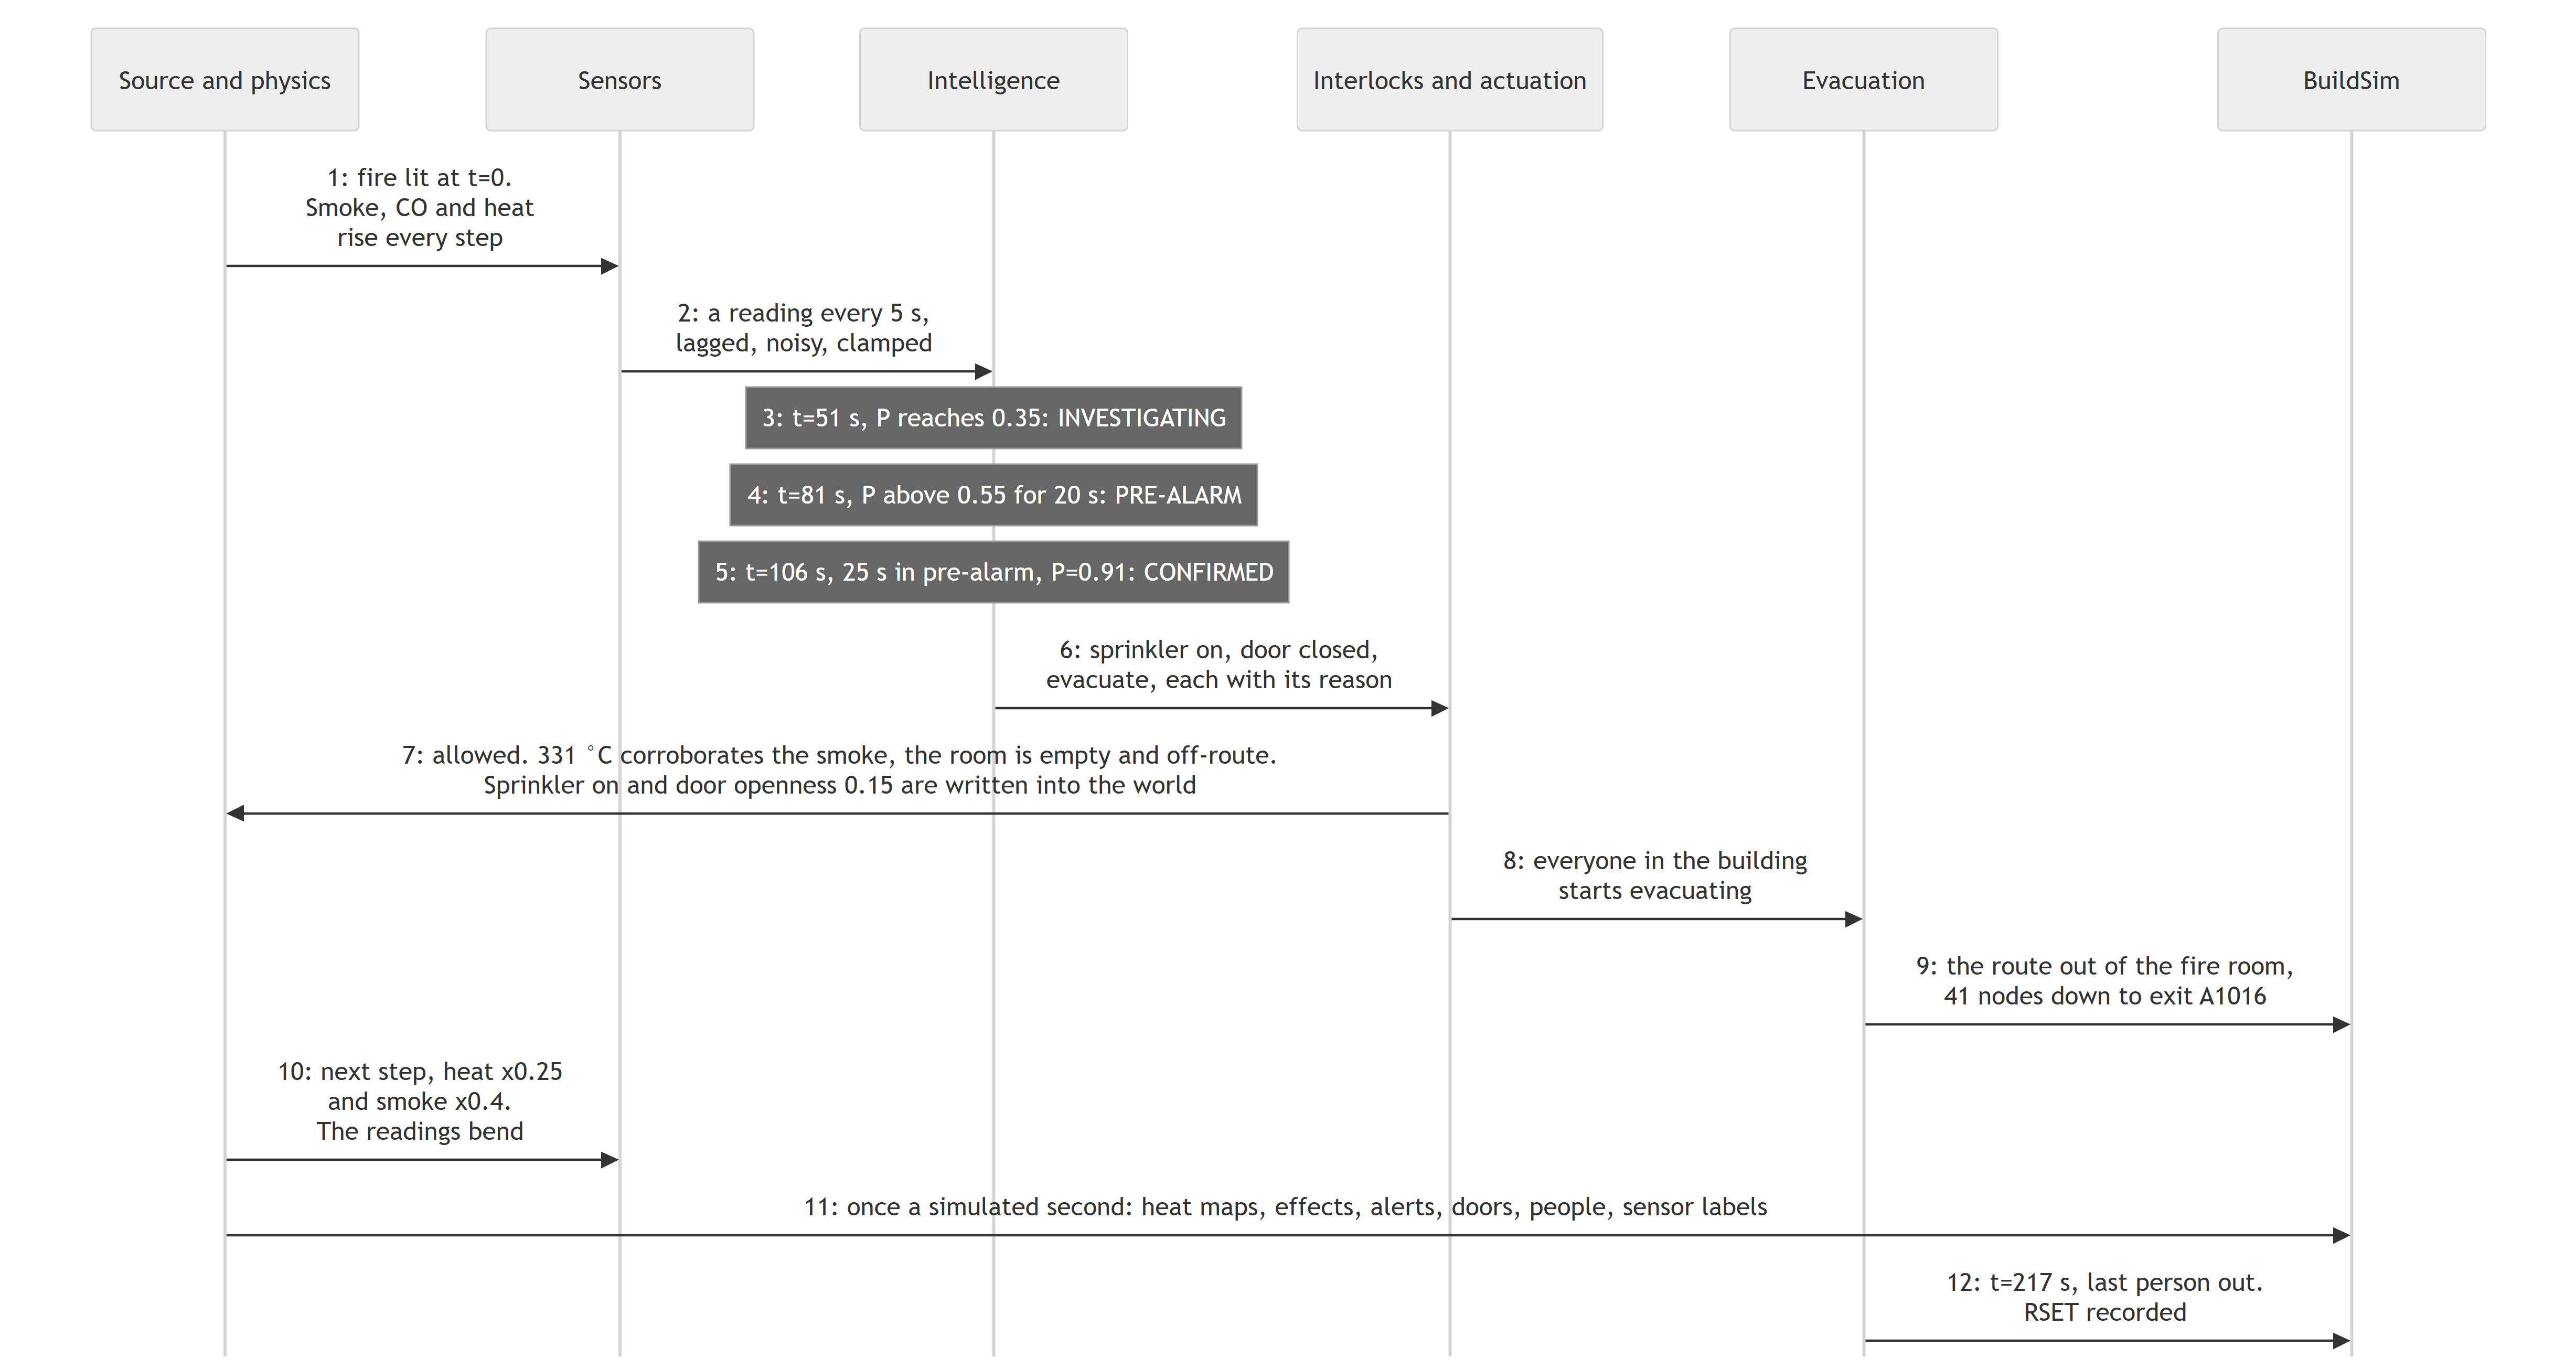
\includegraphics[width=1.00\linewidth]{images/dynamic.png}
\caption{C4 Dynamic diagram of the office fire, with the times measured in Section~11. Steps 3 to 5 are the dwells; step 7 is where the interlocks decide; step 10 is the loop closing.}
\label{fig:dynamic}
\end{figure}

Two things in the order matter. The response is issued and applied in the same
tick that confirms, so nothing waits for the next reading. And the fire door closed
only because A3505 happened to be empty and on nobody's route; had a student been
inside, step~7 would have refused the door, journalled why, and kept the request
pending until they left.

\subsection{8.2 Process lifecycle, state machine}

Every monitored room has one of these, and its transitions are the code in
\code{domain/agent.py}. The dwells are on the arrows.

\begin{figure}[H]
\centering
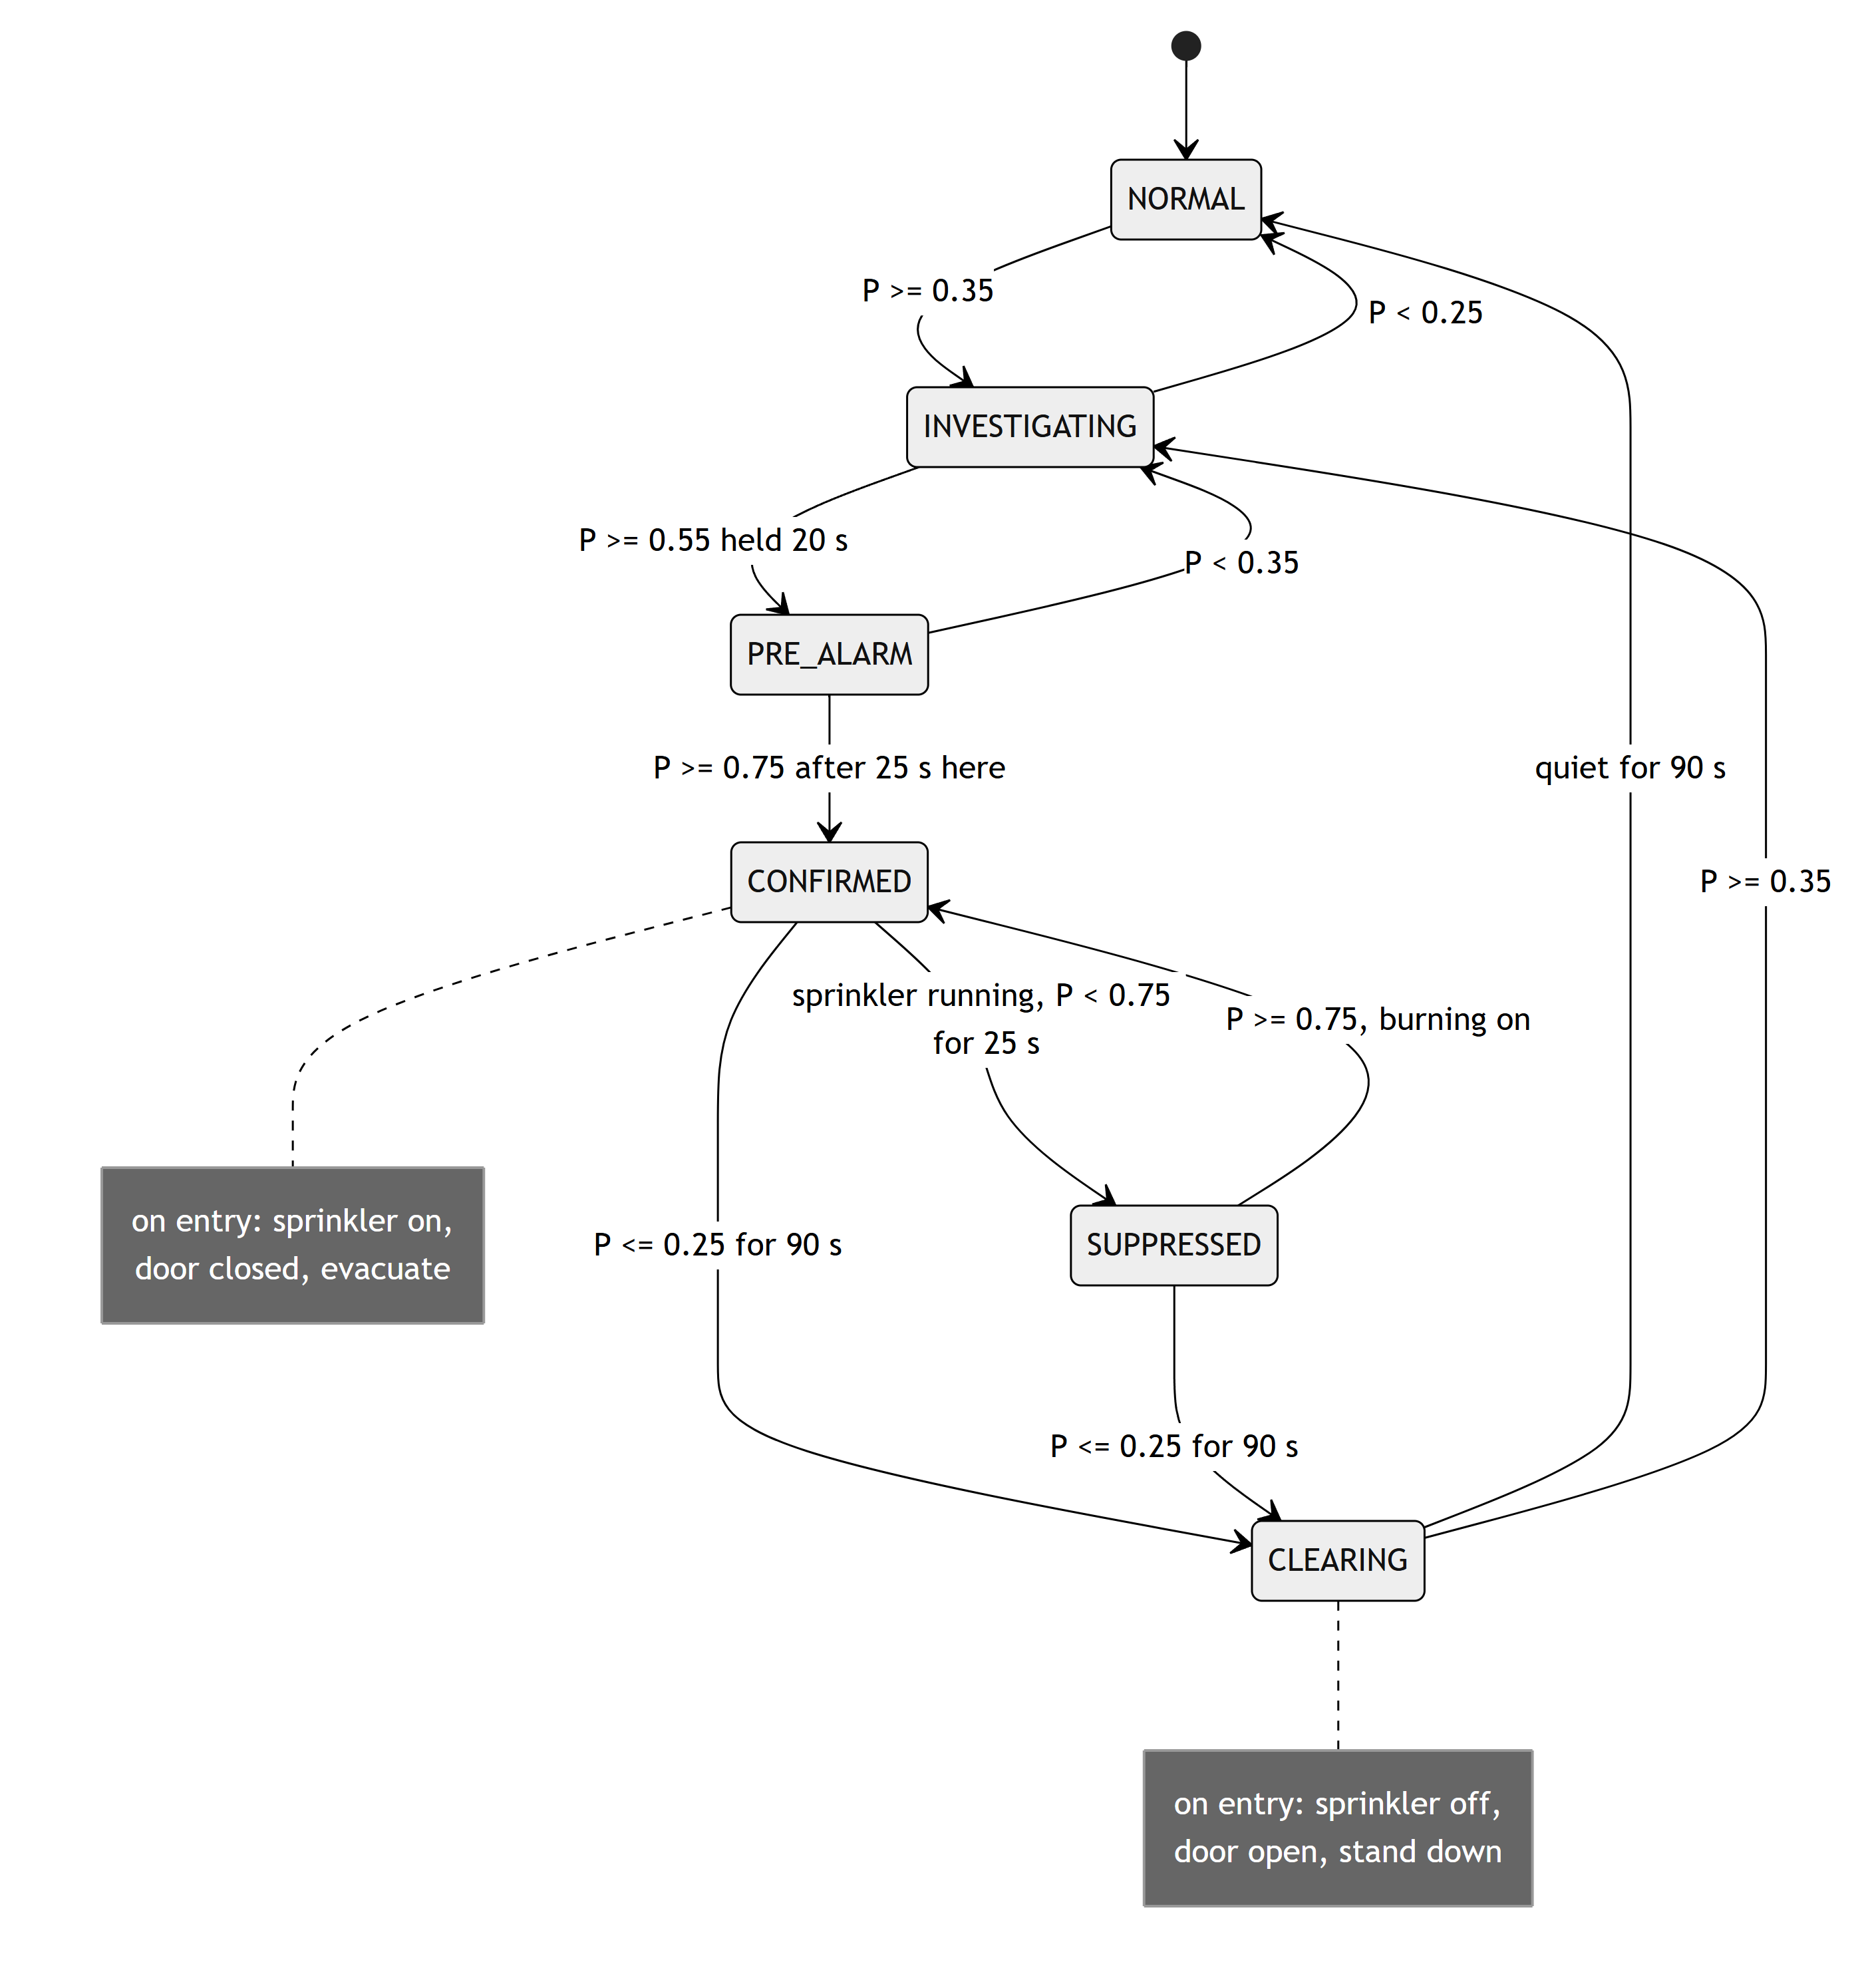
\includegraphics[width=0.72\linewidth]{images/state.png}
\caption{The per-room alarm state machine. Only two states ask for anything; every other arrow only changes what the room believes.}
\label{fig:state}
\end{figure}

\textsc{suppressed} is still an alarm: the fire is being held, not out, and the
confirmed state's outstanding requests stand. A fire that burns on through the
water climbs straight back to \textsc{confirmed}. Standing down needs the
probability to stay at or below 0.25 for 90\,s and then a further 90\,s of quiet
before the room stops being flagged as an incident, so a sensor that recovers for a
moment cannot reopen a door onto a fire. The process itself has a lifecycle of its
own outside this diagram: on startup the service loads the floors from BuildSim and
scatters the population; if BuildSim stops answering, the service marks itself
disconnected, keeps simulating, stops publishing, and waits for a reload rather
than crashing.

\section{Deployment and component placement}\label{sec:deployment}

Everything that matters runs on one laptop. So deployment is about how the
system is built from processes, not where they sit in the world. There are two
processes and two browser tabs. They talk only through the interfaces of
Section~\ref{sec:interfaces}. One optional call leaves the machine. When the language model is the
chosen detector, it runs on a shared server on the university network.

\begin{figure}[H]
\centering
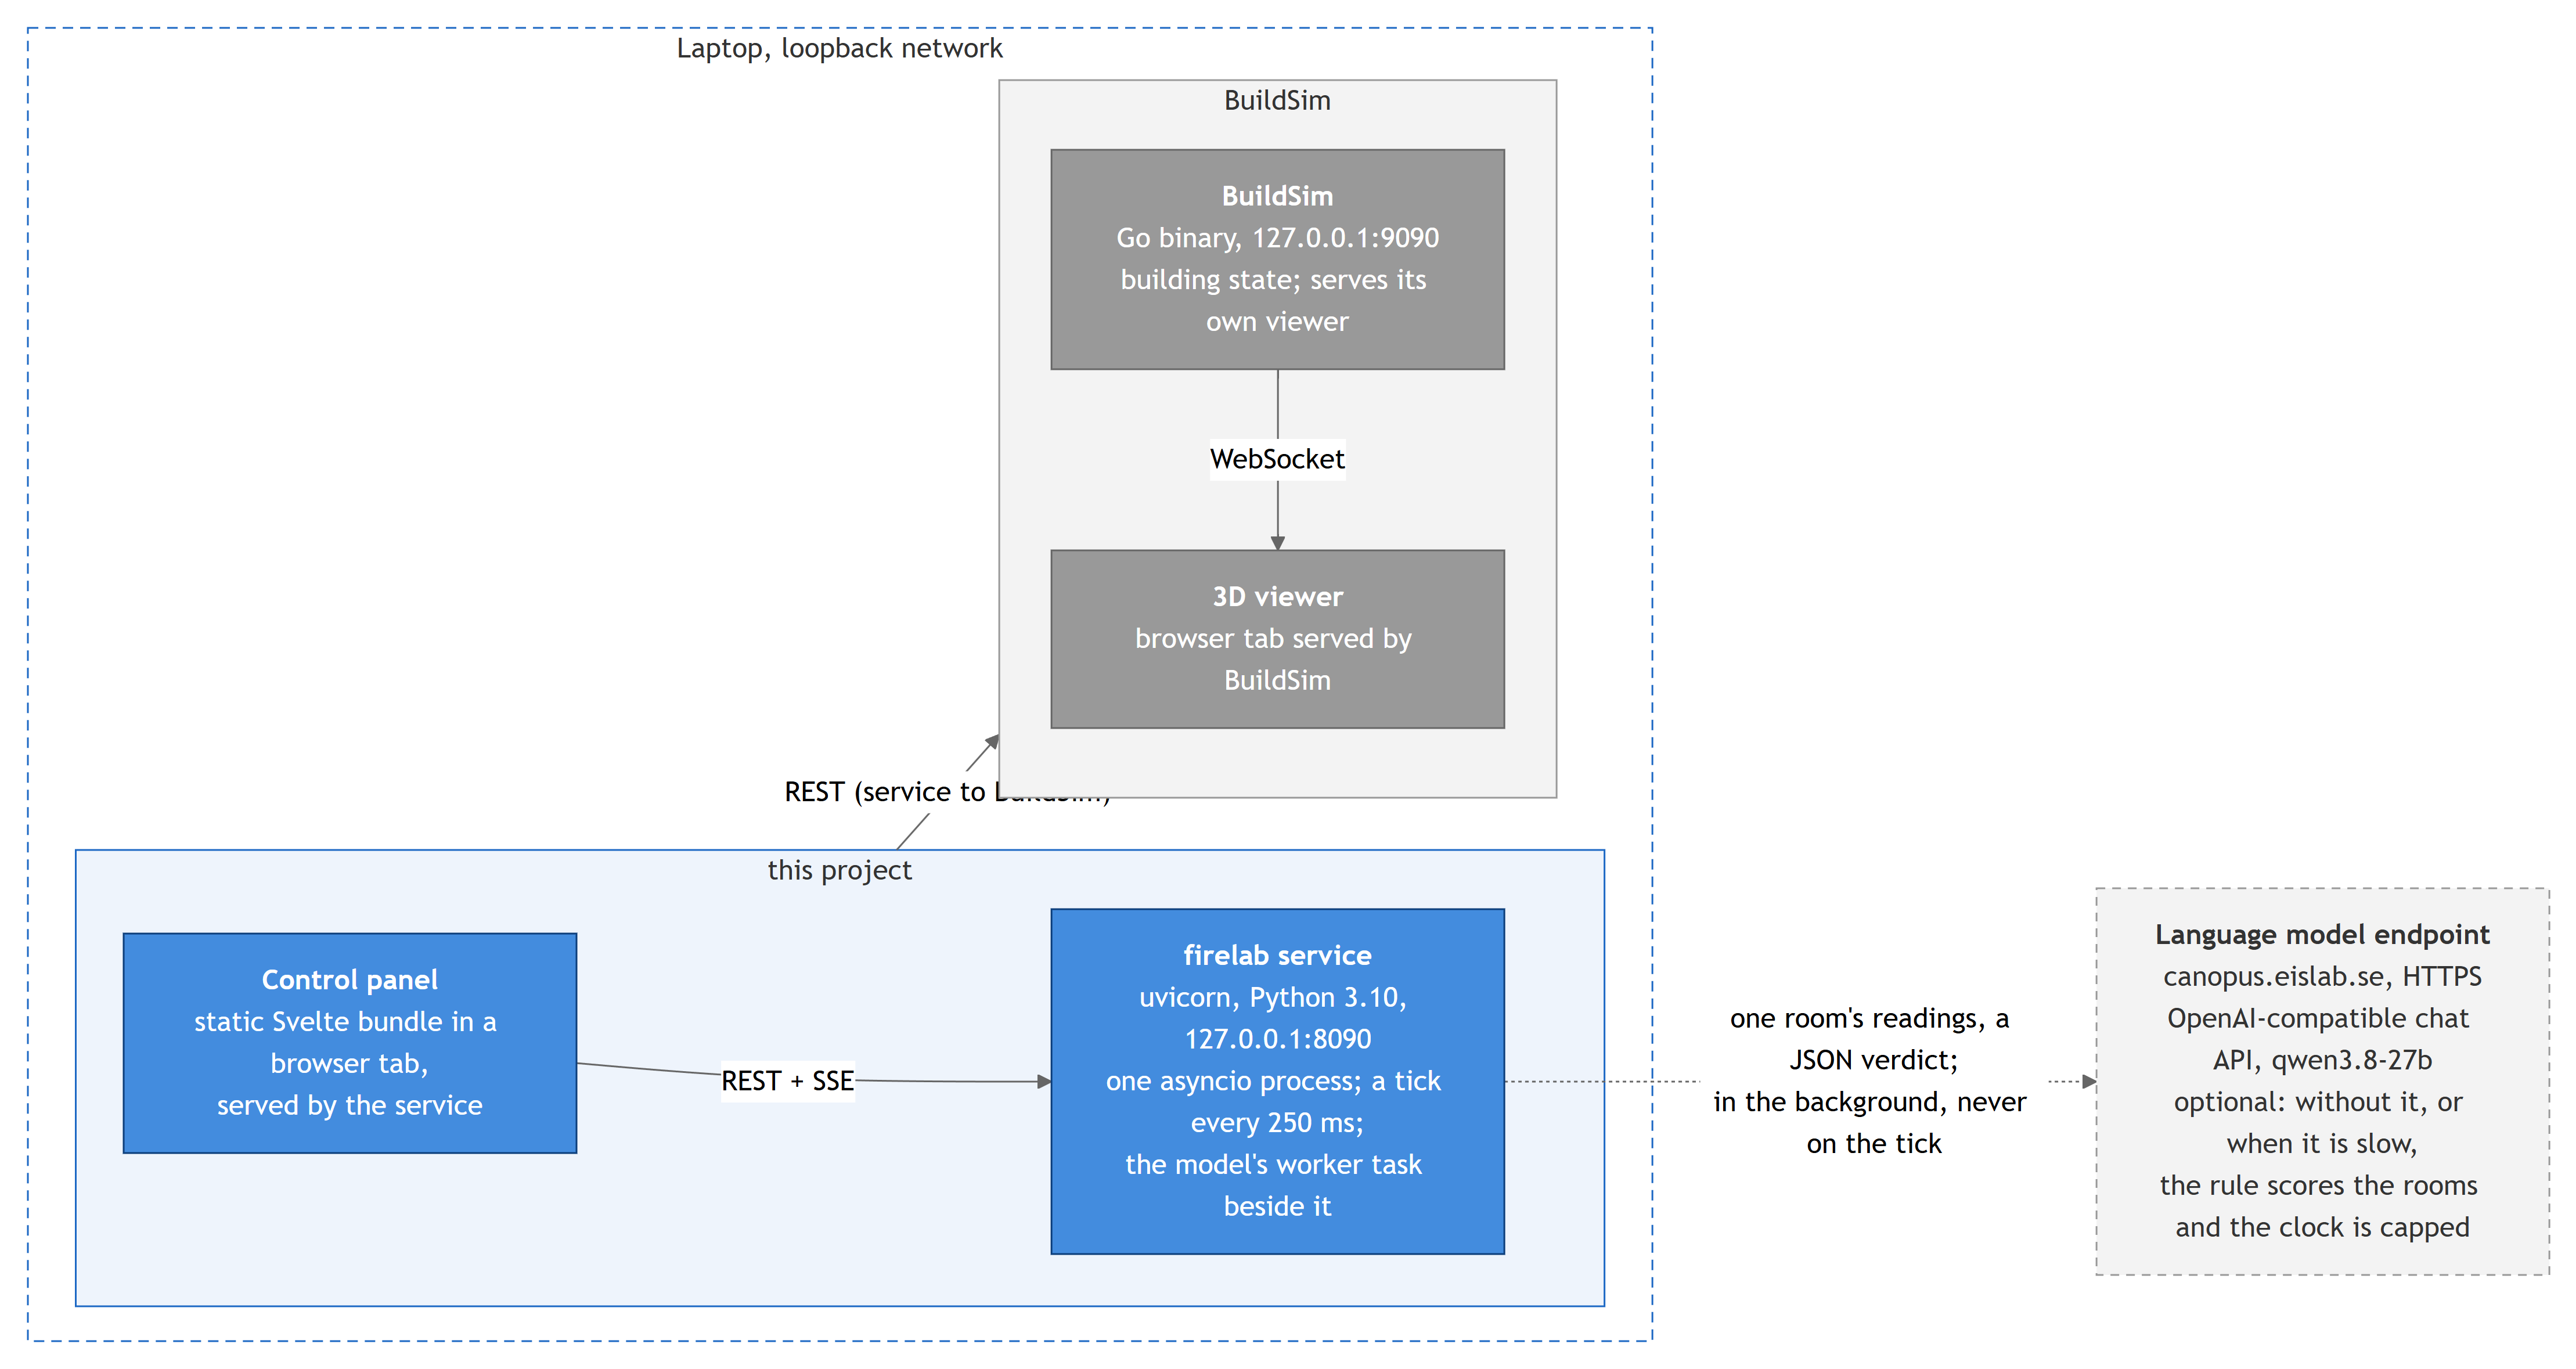
\includegraphics[width=0.95\linewidth]{images/deploy.png}
\caption{Deployment view: two processes, two tabs, loopback only. The purple box, reached by the dotted arrow, is the only part that leaves the laptop. The system keeps detecting without it.}
\label{fig:deploy}
\end{figure}

\textbf{Why this placement.} The control loop lives in the firelab process. It
runs from the physics, through the sensors, to the safety rules (interlocks) and
back. It touches nothing outside the machine except BuildSim over loopback. In a
real building, this process is the edge node. It must keep working when the
internet does not. It must also answer within the tick budget, which Section~\ref{sec:evaluation}
measures. The model endpoint puts that idea to the test. It is off the edge, it
is slow, and someone else runs it. So the adapter treats it as advice, not as
something the system depends on. The rule scores every room the model has not
answered for. The tick never waits for the call. If the endpoint disappears, the
journal says so and nothing else changes. A real building would need this design
for any cloud service on the detection path. That is why the box is dotted.
BuildSim stands in for the building's own controllers, and I left it alone.

\textbf{What is lost by merging the zones into one process}, since the course
asks: fault isolation and independent restart. If the physics crashes, the agent
dies with it. That is fine for a simulator on a laptop, but not for a building.
The safeguard I built in is the layering. It keeps the zones as easy to separate
as separate processes would. I also know where to split. The sensing zone already
produces readings per device, keyed by device ID. The actuation zone already takes
commands with a reason. Those are the two messages a broker would carry.

\textbf{Operational notes.} You start the service with \code{make run}. This
creates a virtual environment, builds the panel and serves it. Configuration is
live. Speed, thresholds, waiting times, sensor noise and population change on the
next tick through \code{PUT /api/config}. A reload re-reads the floors from
BuildSim without a restart. If BuildSim is down at startup, the service says so in
its journal and sits idle until a reload. If BuildSim goes away mid-run, the
service marks itself disconnected and stops writing. It keeps simulating.

\section{Test plan}\label{sec:testplan}

Two kinds of evidence back the requirements. The first is the unit suite: 162
tests and 98 subtests in 22 files. It runs in three seconds with nothing else
running. That works because the domain imports nothing that needs a network. The
model detector is tested against a fake endpoint and a fake clock. The second is
the experiments (E1 to E7). They drive the real engine tick by tick against the
loaded building, with publishing switched off. They use the same seed every time
and write their measurements to \code{experiments/results/}. E7, the model
comparison, is the only one that also needs the endpoint and a wall clock.
Section~\ref{sec:evaluation} reports them.

\begin{longtable}[]{@{}
  >{\raggedright\arraybackslash}p{(\columnwidth - 6\tabcolsep) * \real{0.12}}
  !{\colsep}>{\raggedright\arraybackslash}p{(\columnwidth - 6\tabcolsep) * \real{0.44}}
  !{\colsep}>{\raggedright\arraybackslash}p{(\columnwidth - 6\tabcolsep) * \real{0.16}}
  !{\colsep}>{\raggedright\arraybackslash}p{(\columnwidth - 6\tabcolsep) * \real{0.28}}@{}}
\toprule
\rowcolor{tablehead}
\textbf{ID} & \textbf{Test} & \textbf{Requirement} & \textbf{Evidence} \\
\midrule
\endhead
T-1 & \code{test\_agent}: the ladder climbs one step at a time and respects every waiting time. Only \textsc{confirmed} and \textsc{clearing} send commands & FR-01, FR-04 & unit, passes \\
\rowline
T-2 & \code{test\_detector}: P(fire), the estimated chance of fire in a room, equals the sum of its parts. A room with no sensors gives no opinion. Cooking scores below the confirm threshold & FR-03, FR-06 & unit, passes \\
\rowline
T-3 & \code{test\_interlocks}: water is refused below 35\,°C. Lock is always refused. Close is refused when the room is occupied or on a route & SR-01 to SR-03 & unit, passes \\
\rowline
T-4 & \code{test\_sensing}: lag, rounding (quantisation), clamping and each of the four faults behave as specified & NFR-02 & unit, passes \\
\rowline
T-5 & \code{test\_physics}, \code{test\_sources}: relaxation, the diffusion cap, sprinkler factors, the $t^2$ curve & Section~\ref{sec:physics} & unit, passes \\
\rowline
T-6 & \code{test\_evacuation}, \code{test\_walkways}, \code{test\_multifloor}: clear routes avoid danger, upper floors reach a ground-floor exit, and the drawn route starts at the fire & FR-05 & unit, passes \\
\rowline
T-7 & \code{test\_scoring}, \code{test\_history}: the catch, miss and false-alarm rules. The RSET milestones (RSET is the time from ignition until the last person is out). The recorder's columns and length & FR-07 & unit, passes \\
\rowline
T-8 & \code{test\_layering}: the direction of imports and the truth boundary & NFR-04 & unit, passes \\
\rowline
T-9 & \code{test\_publishing\_route}, \code{test\_publisher\_doors}: the route is sent only when it changes, and it names its storeys. Closed doors reach BuildSim & NFR-05 & unit, passes \\
\rowline
T-10 & \code{test\_reset}, \code{test\_presets}: a reset returns to a quiet building and forgets injected faults. Every preset is well formed & NFR-03 & unit, passes \\
\rowline
T-11 & \code{test\_llm\_detector}: the prompt carries readings only. A good reply becomes an answer, and a bad one is refused. The rule answers until the model has spoken, and again once the model's answer expires. A quiet room costs no question. Each room gets one question at a time, the most suspicious first. The speed limit follows measured answer times & FR-06, FR-08, NFR-06, NFR-07 & unit, passes \\
\rowline
T-12 & \code{test\_pacing}: the rule has no speed limit. A slow detector caps the speed dial once and says so. Switching back lifts the cap & NFR-07 & unit, passes \\
\rowline
E1 & Each of the six presets in A3505 for 20 simulated minutes: state times, score, response, peak truth & FR-01 to FR-04, SR-01 & Table~\ref{tab:presets}, Figure~\ref{fig:office} \\
\rowline
E2 & The office fire with the agent's commands dropped (supervised mode), then with the sprinkler alone & Section~\ref{sec:physics} loop & Table~\ref{tab:contain} \\
\rowline
E3 & Office fire and kitchen cooking at sensor noise 0, 1, 2, 3$\times$ & FR-03, NFR-03 & Table~\ref{tab:noise} \\
\rowline
E4 & Office fire with the smoke detector stuck, dropping out, drifting, or dead & NFR-02 & Table~\ref{tab:faults} \\
\rowline
E5 & Sensors in 10 to 956 rooms; wall time of one tick at 1$\times$ and 40$\times$ & NFR-01 & Figure~\ref{fig:scaling} \\
\rowline
E6 & Every experiment rerun from the same seed & NFR-03 & identical latencies to the second \\
\rowline
E7 & The six presets, cooking at 2 and 3$\times$ noise, and the fire with a stuck smoke detector, scored by the language model at the speed it can keep up with & FR-08, NFR-06, NFR-07 & Table~\ref{tab:detectors}, Figure~\ref{fig:detectors} \\
\bottomrule
\end{longtable}

\section{Evaluation and experiments}\label{sec:evaluation}

This section reports what I measured. The experiment harness in
\code{experiments/run\_experiments.py} measured every number below. It ran on the
loaded A-building, with the fire in office A3505 on the top floor. There were 130
people, placed by the default seed, and the thresholds were the defaults. The fire
room and its neighbours had all three sensor types, as the presets do.

\textbf{Detection and response (E1).}

\begin{table}[H]
\centering
\footnotesize
\resizebox{\linewidth}{!}{\begin{tabular}{@{}l!{\colsep}c!{\colsep}c!{\colsep}c!{\colsep}c!{\colsep}c!{\colsep}c!{\colsep}c@{}}
\toprule
\rowcolor{tablehead}
\textbf{Preset} & \textbf{Investigating} & \textbf{Confirmed} & \textbf{Max P(fire)} & \textbf{False alarms} & \textbf{Sprinkler} & \textbf{RSET} & \textbf{Outcome} \\
\midrule
Office fire (flaming, fast) & 51\,s & 106\,s & 0.994 & 0 & on at 106\,s & 217\,s & caught ✓ \\
\rowline
Overnight smoulder & 136\,s & 201\,s & 0.991 & 0 & refused 201\,s, on 219\,s & 312\,s & caught ✓ \\
\rowline
Kitchen cooking & 326\,s & never & 0.688 & 0 & & & correctly ignored ✓ \\
\rowline
Dust storm & never & never & 0.129 & 0 & & & correctly ignored ✓ \\
\rowline
Fire, dead smoke detector & 61\,s & never (room); 156\,s (neighbour) & 0.748 & 0 & on next door & 267\,s & caught by the neighbour, see below \\
\rowline
Drifting sensor, no fire & never & never & 0.057 & 0 & & & correctly ignored ✓ \\
\bottomrule
\end{tabular}}
\caption{One run of each preset. Times are in seconds since ignition. RSET runs from ignition until the last of 130 people is out. In every caught case, the building was empty 111\,s after the alarm.}
\label{tab:presets}
\end{table}

Both fires were confirmed well within the 180\,s and 300\,s limits of FR-01 and
FR-02. None of the three no-fire presets (cooking, dust and the drifting sensor)
raised an alarm (FR-03). Figure~\ref{fig:office} shows the office fire as the
system saw it. The truth and the reading agree until the heat detector maxes out
at 250\,°C. The probability climbs through the three thresholds. The waiting
times show as the flat time between crossing a level and changing state. After the
sprinkler starts at 106\,s, the true smoke bends down. The temperature keeps
rising in the now sealed room. The smoulder shows the safety rules at work. It was
confirmed on CO with the room at 34\,°C. Its sprinkler request was refused for
lack of heat, and the journal logged this. The request was granted 18\,s later,
when the room passed 35\,°C. The design worked as intended, but the number
deserves a second look. A limit of 35\,°C is a low bar for ``heat
corroboration'' (backing from a heat reading). A warm summer office would pass it.

\begin{figure}[H]
\centering
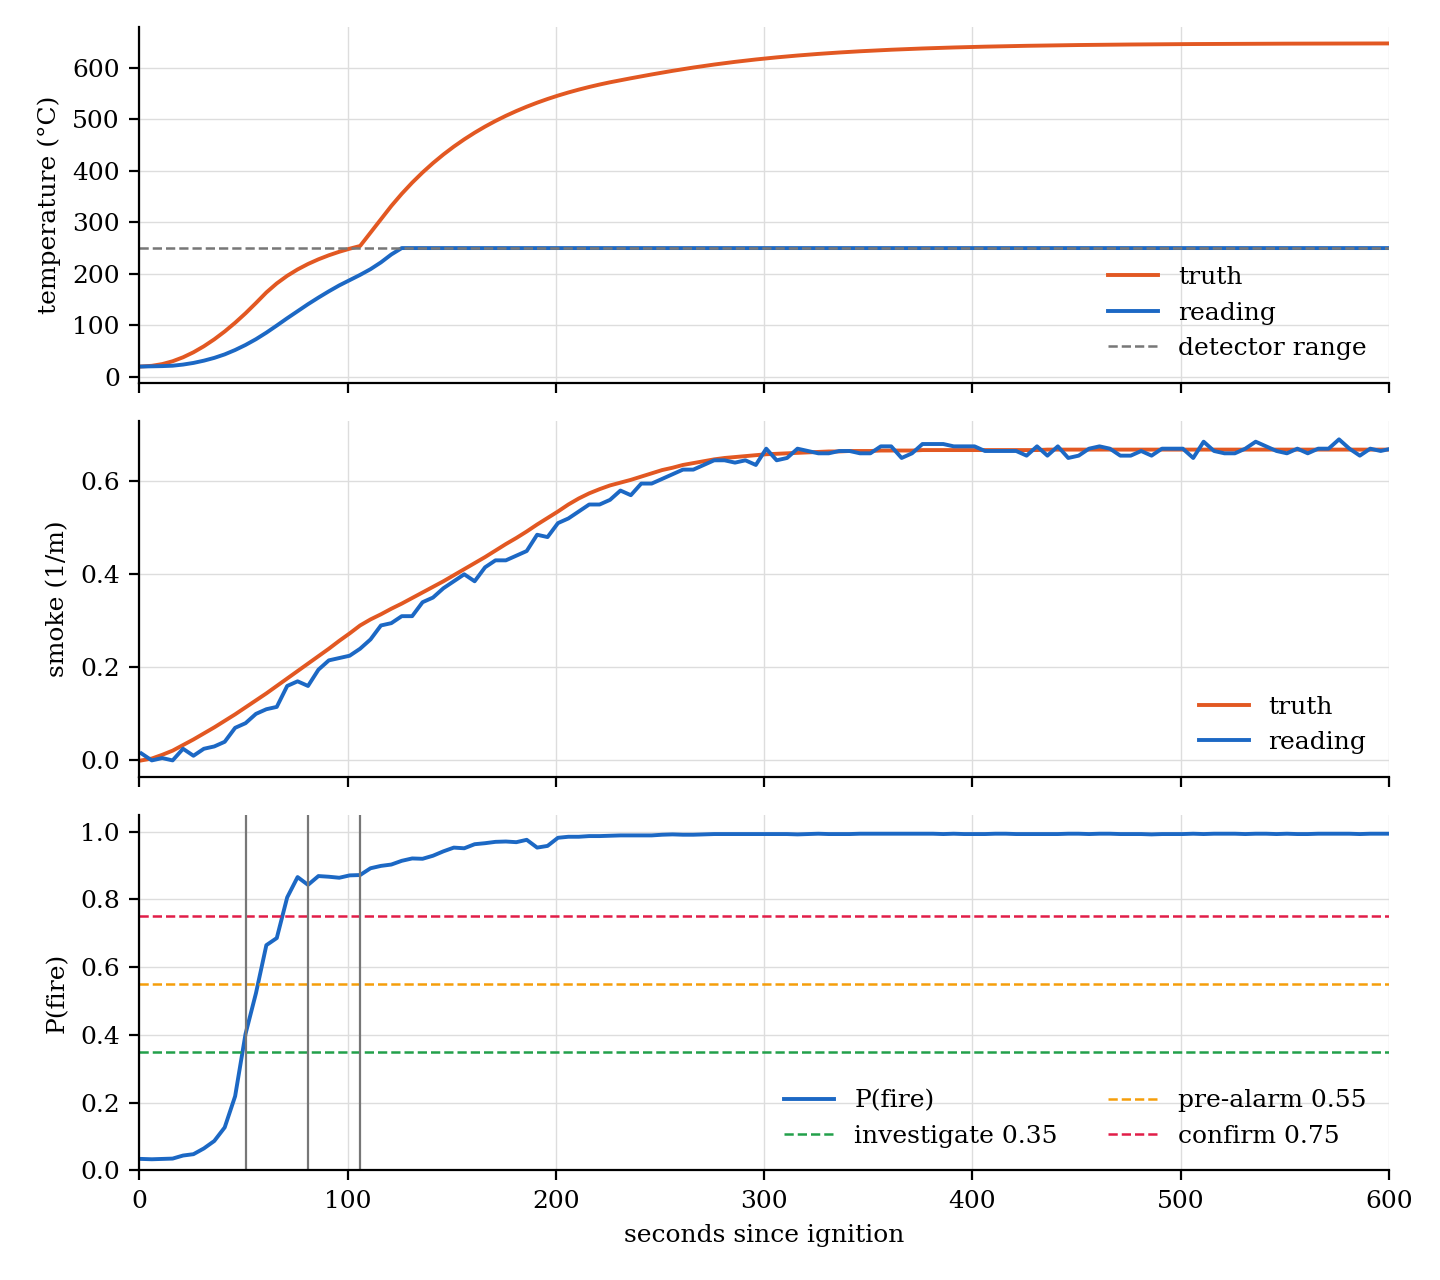
\includegraphics[width=0.92\linewidth]{images/chart_office_fire.png}
\caption{The first ten minutes of the office fire in A3505, as the system saw it (E1). Top: the heat detector maxes out at 250\,°C while the room reaches 648\,°C. Middle: smoke. The reading follows the truth with a 12\,s lag. Bottom: P(fire) passing the three thresholds. The vertical lines are the state changes at 51, 81 and 106\,s. The flat stretches before them are the waiting times.}
\label{fig:office}
\end{figure}

\textbf{The blind spot.} The preset with a dead smoke detector is the one result
that did not go to plan. Heat and CO alone pushed the fire room to a probability of
0.748. The coverage factor held it there. This factor caps a room with two working
sensor types at 85\,\% of its logistic score. The confirm threshold is 0.75. So
the room sat in \textsc{pre-alarm} for the whole run, three thousandths short. The
building was still evacuated at 156\,s. Smoke crossed into A3500A next door, and
its three working detectors confirmed. The fire room also fed A3500A's
neighbour-agreement term. I took two lessons from this. First, the neighbour
cross-check is not decoration: it is what caught this fire. Second, the coverage
penalty is tuned slightly too hard. Two changes would have confirmed the room
itself. One is lowering the penalty by raising its floor from 0.55 to 0.60. The
other is letting a neighbour's confirmation lift the room. This is the first
change I would make.

\textbf{Closing the loop, and what containment actually does (E2).}

\begin{table}[H]
\centering
\footnotesize
\resizebox{\linewidth}{!}{\begin{tabular}{@{}l!{\colsep}c!{\colsep}c!{\colsep}c!{\colsep}c!{\colsep}c@{}}
\toprule
\rowcolor{tablehead}
\textbf{Response} & \textbf{Rooms lost} & \textbf{Neighbour peak smoke} & \textbf{Neighbour peak temp} & \textbf{Fire room peak temp} & \textbf{RSET} \\
\midrule
None (supervised, nobody presses) & 5 & 0.382\,1/m & 149\,°C & 309\,°C & no evacuation \\
\rowline
Autonomous & 4 & 0.171\,1/m & 152\,°C & 648\,°C & 217\,s \\
\rowline
Sprinkler only, door held open & 5 & 0.171\,1/m & 152\,°C & 648\,°C & 217\,s \\
\bottomrule
\end{tabular}}
\caption{The same office fire three times. ``Rooms lost'' are rooms that became untenable at any point in 20 minutes. Untenable means unsafe for people to stay in, judged by the limits in the ISO 13571 standard.}
\label{tab:contain}
\end{table}

The response halves the smoke that reaches the neighbours and saves one room. It
also makes the fire room hotter. That surprised me until the journal explained it.
With the door open, the fire room dumps heat into five neighbours every step. With
the doors closed, it keeps the heat. The sprinkler's 25\,\% factor does not make
up for that. In this model, water reduces the heat the fire releases. It does
nothing to cool the room directly. The third row tells me more. Holding the fire
room's own door open made no difference at all. At 231\,s the neighbour A3500A
confirmed on the smoke that had crossed into it. It then closed \emph{its} doors,
and one of them is the same doorway. So in this building, containment depends on
every room around the fire, not on the fire room alone. Without any response,
nobody is told to leave and no RSET is recorded. That is the simplest argument for
making the evacuate command automatic.

\textbf{Noise (E3) and lying sensors (E4).}

\begin{table}[H]
\centering
\footnotesize
\begin{minipage}[t]{0.47\linewidth}
\centering
\begin{tabular}{@{}l!{\colsep}c!{\colsep}c!{\colsep}c!{\colsep}c@{}}
\toprule
\rowcolor{tablehead}
\textbf{Noise} & \multicolumn{2}{c}{\textbf{Office fire}} & \multicolumn{2}{c}{\textbf{Kitchen cooking}} \\
\rowcolor{tablehead}
 & confirmed & max P & alarms & max P \\
\midrule
0$\times$ & 106\,s & 0.994 & 0 & 0.447 \\
\rowline
1$\times$ & 106\,s & 0.994 & 0 & 0.688 \\
\rowline
2$\times$ & 106\,s & 0.995 & 0 & 0.749 \\
\rowline
3$\times$ & 106\,s & 0.996 & 0 & 0.741 \\
\bottomrule
\end{tabular}
\caption{Sensor noise sweep (E3).}
\label{tab:noise}
\end{minipage}\hfill
\begin{minipage}[t]{0.47\linewidth}
\centering
\begin{tabular}{@{}l!{\colsep}c!{\colsep}c@{}}
\toprule
\rowcolor{tablehead}
\textbf{Smoke detector} & \textbf{Confirmed} & \textbf{Max P} \\
\midrule
healthy & 106\,s & 0.994 \\
\rowline
dropout (40\,\% lost) & 101\,s & 0.995 \\
\rowline
drift & 106\,s & 0.995 \\
\rowline
stuck & 156\,s & 0.880 \\
\rowline
dead & never (neighbour 156\,s) & 0.748 \\
\bottomrule
\end{tabular}
\caption{Faults on the fire room's smoke detector during the office fire (E4).}
\label{tab:faults}
\end{minipage}
\end{table}

Detection time did not move by a second across the noise sweep, and cooking never
raised an alarm. That is the waiting times doing their job. The number to worry
about is the cooking peak at 2$\times$ noise: 0.749 against a confirm threshold of
0.75. It did not confirm. To confirm, it would first have to hold 0.55 for 20\,s
and then sit 25\,s in pre-alarm, and it never did. But the margin on the
probability itself is only one noise sample wide. The CO term is what keeps
cooking down. So, to be accurate, this detector tells cooking from fire by CO and
time, not by any single reading. On faults, a detector that dropped readings
caught the fire slightly faster. The readings it did send happened to land on
rising edges. A stuck detector cost 50\,s, because the rate term went flat. Drift
did nothing in twenty minutes. A dead detector is the blind spot above.

\textbf{Scaling and the breaking point (E5).} The tick loop wakes every 250\,ms
of real time. It must finish before it wakes again. At 1$\times$ speed, one tick is
one physics step over the whole building plus one intelligence pass over the
monitored rooms. At 40$\times$ it is forty physics steps and one pass.

\begin{figure}[H]
\centering
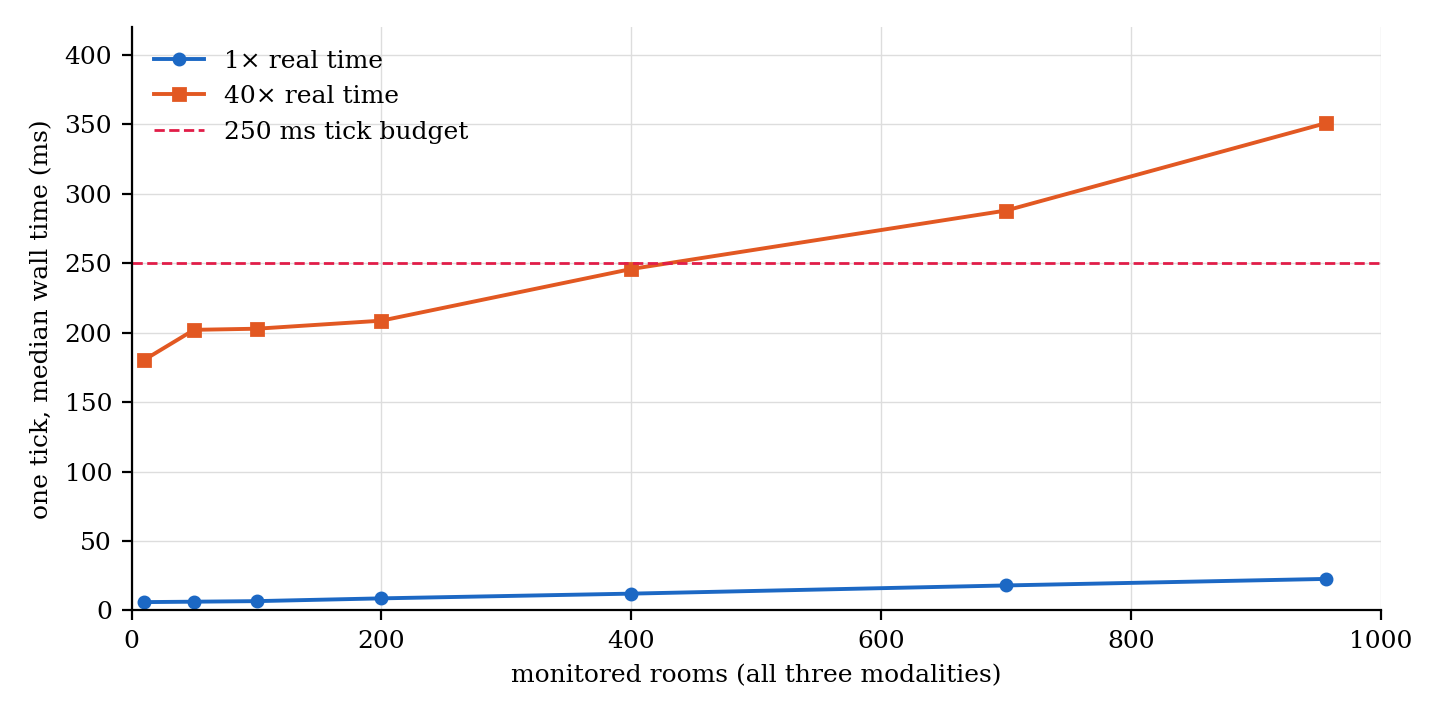
\includegraphics[width=0.86\linewidth]{images/chart_scaling.png}
\caption{Real (wall-clock) time of one engine tick against the number of monitored rooms (E5), on the laptop the demo runs on. The building has 956 rooms and 1005 doorways.}
\label{fig:scaling}
\end{figure}

At real time the whole building fits with room to spare: 23\,ms per tick with all
956 rooms monitored and 2868 devices sampling. At 40$\times$ the tick goes over
budget at about 450 monitored rooms. The shape of the curve shows where the cost
is. With only 10 rooms monitored, a 40$\times$ tick already takes 180\,ms. So the
forty physics steps over the full graph are the fixed cost, about 4.5\,ms a step.
The intelligence adds about 0.18\,ms per monitored room on top. The physics cost
does not grow with the number of sensors. So for a bigger building or a faster
clock, the fix is a sparser diffusion step, not a faster detector. When the tick
goes over budget, nothing breaks. The loop just runs slower than the speed dial
claims. The tick also caps itself at sixty physics steps, so a stall cannot
snowball.

\textbf{The language model as the detector (E7).} I ran the same scenarios again
with the language model (\code{qwen3.8-27b} on the lab's server) deciding P(fire)
instead of the rule. The script is \code{experiments/compare\_detectors.py}. The
model is asked about one room at a time, and each answer is trusted for 60
simulated seconds. When the model has no recent answer, the rule fills in. So the
numbers below are for the model and the rule working together, not the model on
its own. These runs are slow because they wait for real answers: the nine of them
took 98 minutes.

\begin{table}[H]
\centering
\footnotesize
\resizebox{\linewidth}{!}{\begin{tabular}{@{}l!{\colsep}c!{\colsep}c!{\colsep}c!{\colsep}c!{\colsep}c!{\colsep}c!{\colsep}c!{\colsep}c@{}}
\toprule
\rowcolor{tablehead}
\textbf{Scenario} & \textbf{Rule: alarm} & \textbf{Model: alarm} & \textbf{Model max P} & \textbf{Model share} & \textbf{Answered / failed / asked} & \textbf{Median answer} & \textbf{Clock} \\
\midrule
Office fire & 106\,s & 136\,s & 0.99 & 57\,\% & 32 / 2 / 35 & 7.3\,s & 2.5$\times$ \\
\rowline
Overnight smoulder & 201\,s & 201\,s & 0.97 & 32\,\% & 16 / 5 / 22 & 14.8\,s & 2.3$\times$ \\
\rowline
Kitchen cooking, 1$\times$ noise & none & none & 0.22 & 39\,\% & 33 / 1 / 36 & 14.5\,s & 2.0$\times$ \\
\rowline
Kitchen cooking, 2$\times$ noise & none & none & 0.72 & 38\,\% & 33 / 2 / 36 & 15.1\,s & 2.0$\times$ \\
\rowline
Kitchen cooking, 3$\times$ noise & none & none & 0.76 & 43\,\% & 35 / 1 / 37 & 17.3\,s & 1.8$\times$ \\
\rowline
Dust storm & none & none & 0.07 & 92\,\% & 36 / 0 / 36 & 7.2\,s & 3.0$\times$ \\
\rowline
Fire, dead smoke detector & 156\,s (neighbour) & 156\,s (neighbour); room 798\,s & 0.90 & 18\,\% & 22 / 3 / 26 & 21.5\,s & 2.1$\times$ \\
\rowline
Drifting sensor, no fire & none & none & 0.08 & 86\,\% & 43 / 0 / 45 & 7.9\,s & 3.0$\times$ \\
\rowline
Office fire, stuck smoke detector & 156\,s & 156\,s & 0.93 & 57\,\% & 37 / 4 / 42 & 20.0\,s & 1.4$\times$ \\
\bottomrule
\end{tabular}}
\caption{The rule compared with the language model (E7). Alarm: when the first room in the building was confirmed, in seconds after the fire started. Model share: how much of the time the model, not the rule, was scoring the fire room. Clock: how fast the simulation could run so the model's answers were still fresh when they arrived.}
\label{tab:detectors}
\end{table}

\begin{figure}[H]
\centering
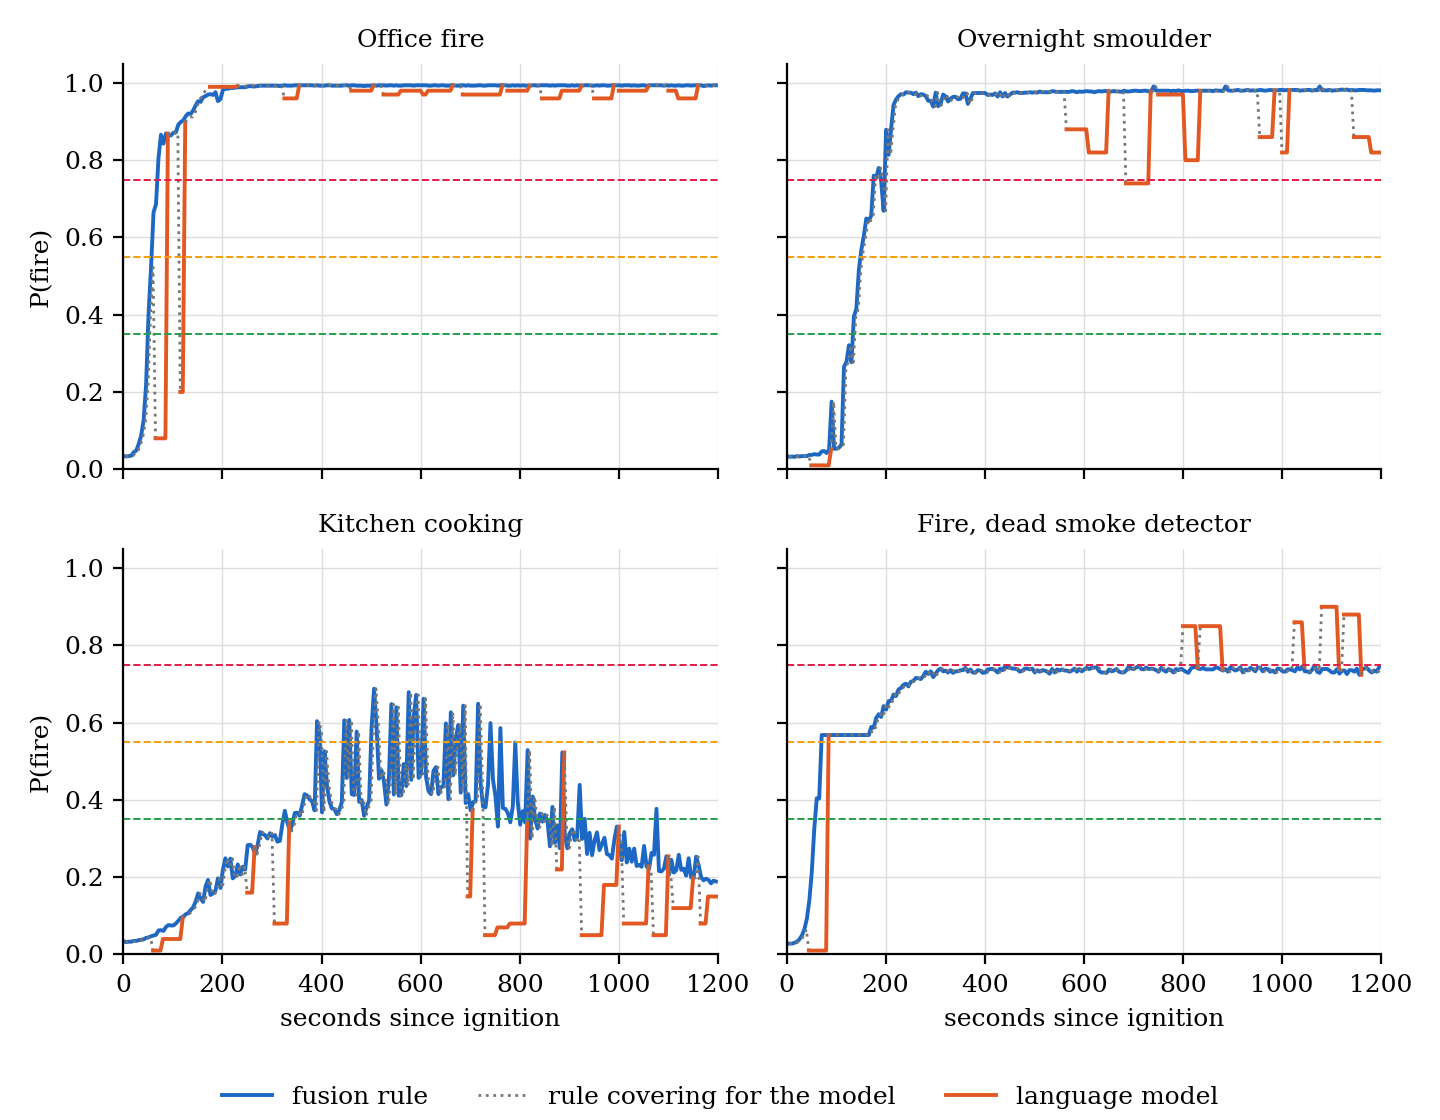
\includegraphics[width=0.92\linewidth]{images/chart_detectors.png}
\caption{P(fire) in the fire room with each detector (E7). Blue: the rule on its own. Orange: the model's answers. Grey dots: the rule filling in while the model had no recent answer. The dashed lines are the three alarm levels.}
\label{fig:detectors}
\end{figure}

In all nine runs the end result was the same as with the rule: every fire was
caught and nothing else set off an alarm. The differences are in how fast, and in
what it cost.

In the office fire, the model's first answers were low. Twice, at 64\,s and
116\,s, they sent the fire room back to \textsc{normal}, and the waiting time
started over. The alarm came 30\,s later than with the rule, and it came from the
room next door (A3500A). The fire room itself was confirmed at 170\,s.

With the dead smoke detector, the model did something the rule could not. It gave
the fire room 0.85 to 0.90, while the rule got stuck at 0.748, so the model
confirmed the room itself. But its answers about that room came so slowly that
this only happened at 798\,s. By then the room next door had already raised the
alarm, at 156\,s, in both runs.

For cooking, the model was calmer than the rule at normal noise (0.22 against
0.688). At three times the noise it was not: it reached 0.76, just over the
confirm level. The waiting times stopped it from raising an alarm, just as they
did for the rule.

The real cost is speed. A typical answer took 7 to 21\,s, and the slowest took
85\,s. 18 of 315 questions failed. The simulation could only run 1.4 to 3 times
faster than real time, while the rule manages 40 times. In the quiet runs the
model was scoring the fire room 86 to 92\,\% of the time, but in the fires only 18
to 57\,\%. So in the runs that mattered most, the rule did a lot of the work. The
results also change from run to run, even with the same seed, because what the
model is asked depends on how long its last answer took.

What the model gave me was a second opinion where the rule was too strict, and a
reason in the journal that a person can read. What it could not do was make
things worse than a delay. The waiting times, the safety rules and the rule
filling in all sit between the model's number and anything that happens in the
building.

\textbf{Headline results.}

\begin{table}[H]
\centering
\footnotesize
\resizebox{\linewidth}{!}{\begin{tabular}{@{}l!{\colsep}l!{\colsep}l!{\colsep}l@{}}
\toprule
\rowcolor{tablehead}
\textbf{Metric} & \textbf{Measured} & \textbf{Requirement} & \\
\midrule
Flaming fire confirmed & 106\,s & $\le 180$\,s (FR-01) & ✓ \\
\rowline
Smouldering fire confirmed & 201\,s & $\le 300$\,s (FR-02) & ✓ \\
\rowline
False alarms, 3 no-fire presets $\times$ 4 noise levels & 0 & 0 (FR-03) & ✓ \\
\rowline
Commands on confirmation & sprinkler, door, evacuate, same tick, with reasons & (FR-04) & ✓ \\
\rowline
Sprinkler refused without heat & yes, released 18\,s later & (SR-01) & ✓ \\
\rowline
Fire caught with a stuck, dropping or drifting smoke detector & yes, worst 156\,s & (NFR-02) & ✓ \\
\rowline
Fire room confirmed with a dead smoke detector & no; caught next door at 156\,s & (NFR-02) & partial \\
\rowline
Tick at 1$\times$, full building & 23\,ms & $\le 250$\,ms (NFR-01) & ✓ \\
\rowline
Breaking point at 40$\times$ & about 450 monitored rooms & measured (NFR-01) & ✓ \\
\rowline
Building of 130 cleared after the alarm & 111\,s & reported (FR-07) & ✓ \\
\rowline
Same seed, same run & identical to the second, every rerun & (NFR-03) & ✓ \\
\rowline
Language model as detector, 9 scenarios & all 4 fires caught, 0 false alarms & (FR-08) & ✓ \\
\rowline
Model answers never used when out of date & typical answer 7--21\,s; simulation held to 1.4--3$\times$ & (NFR-07) & ✓ \\
\bottomrule
\end{tabular}}
\end{table}

\section{Dashboard}\label{sec:dashboard}

The dashboard is two browser tabs. They are meant to be read together, and each
has its own job. The BuildSim viewer shows the building. It has heat maps of the
true temperature, smoke and CO on the floors. It shows flames and smoke in the
burning room, the sprinkler running, and every one of the 130 people walking.
Alarming rooms are outlined in red, orange or yellow by state. The one escape
route is a red line from the fire room, down the stairs, to a ground-floor exit.
The control panel shows the system: what it is told, what it believes, and what
it did about it.

\begin{figure}[H]
\centering
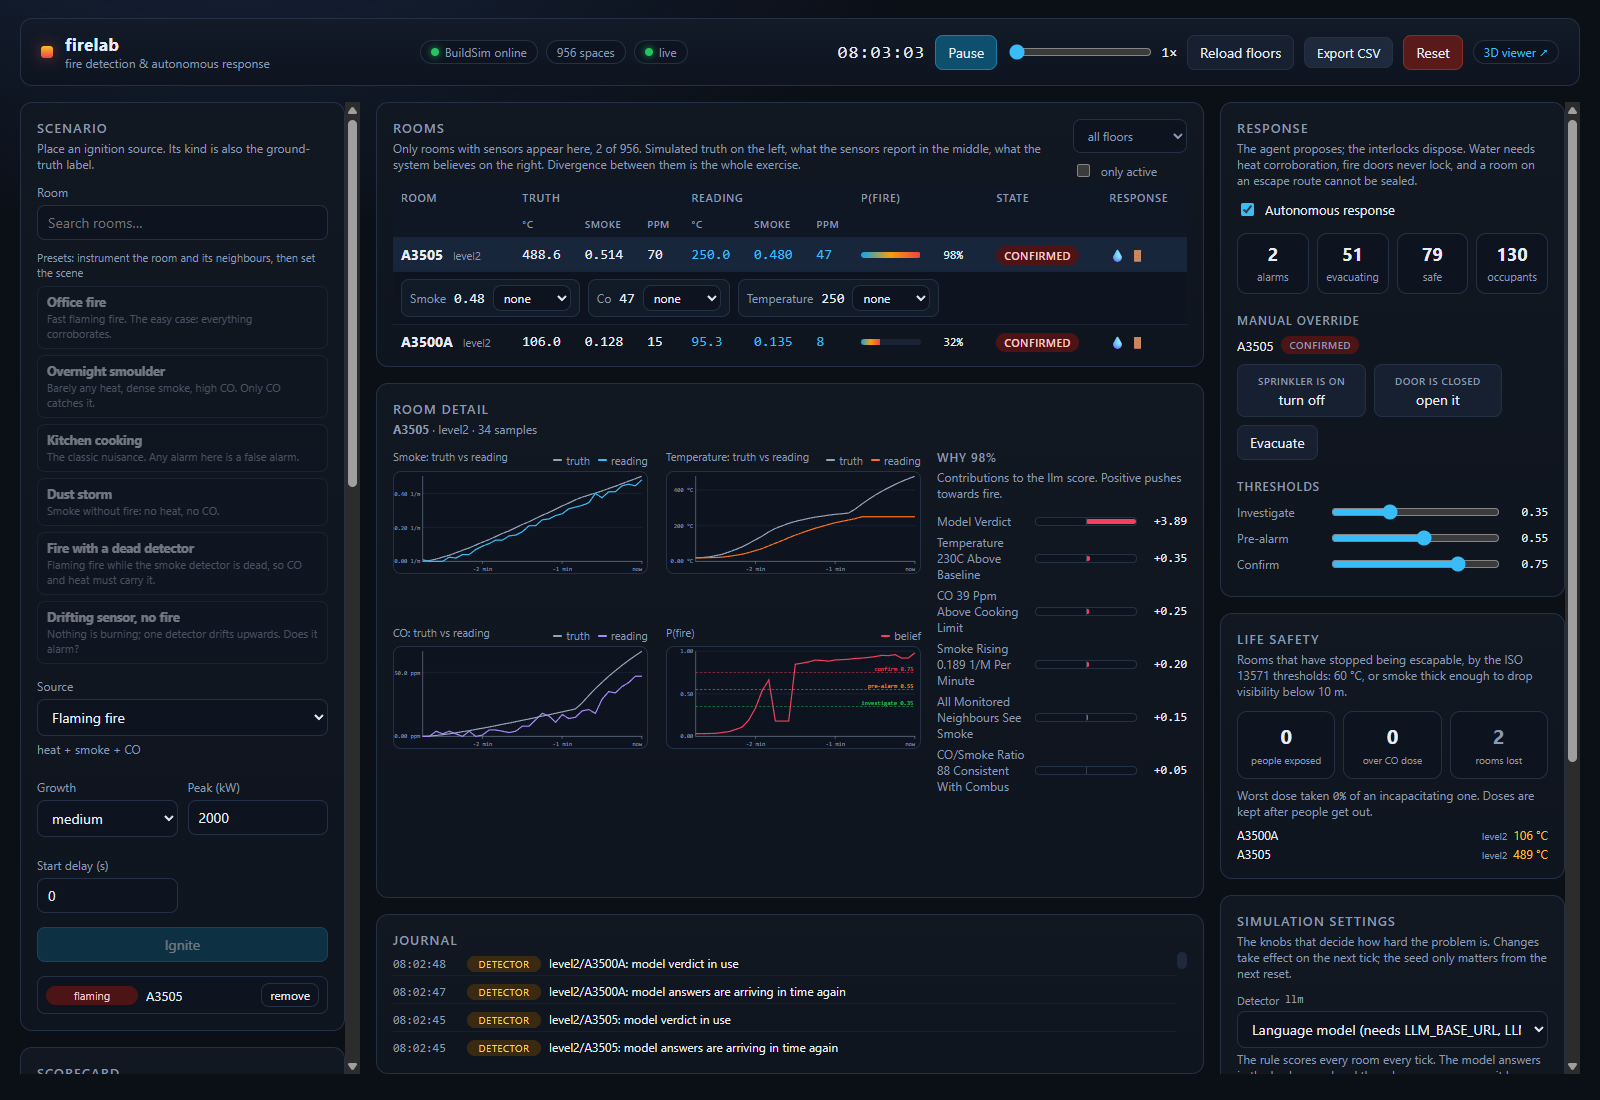
\includegraphics[width=\linewidth]{images/dashboard.png}
\caption{The control panel during the office fire, with the language model as the detector. Rooms table: truth on the left, readings in the middle, P(fire) and state on the right. Room detail: truth against reading for each sensor type, and the ``Why'' bars. Here the bars show the model's own evidence, with its answer as the top bar. Journal: the model's hand-overs. Bottom right: the detector selector.}
\label{fig:dashboard}
\end{figure}

\begin{figure}[H]
\centering
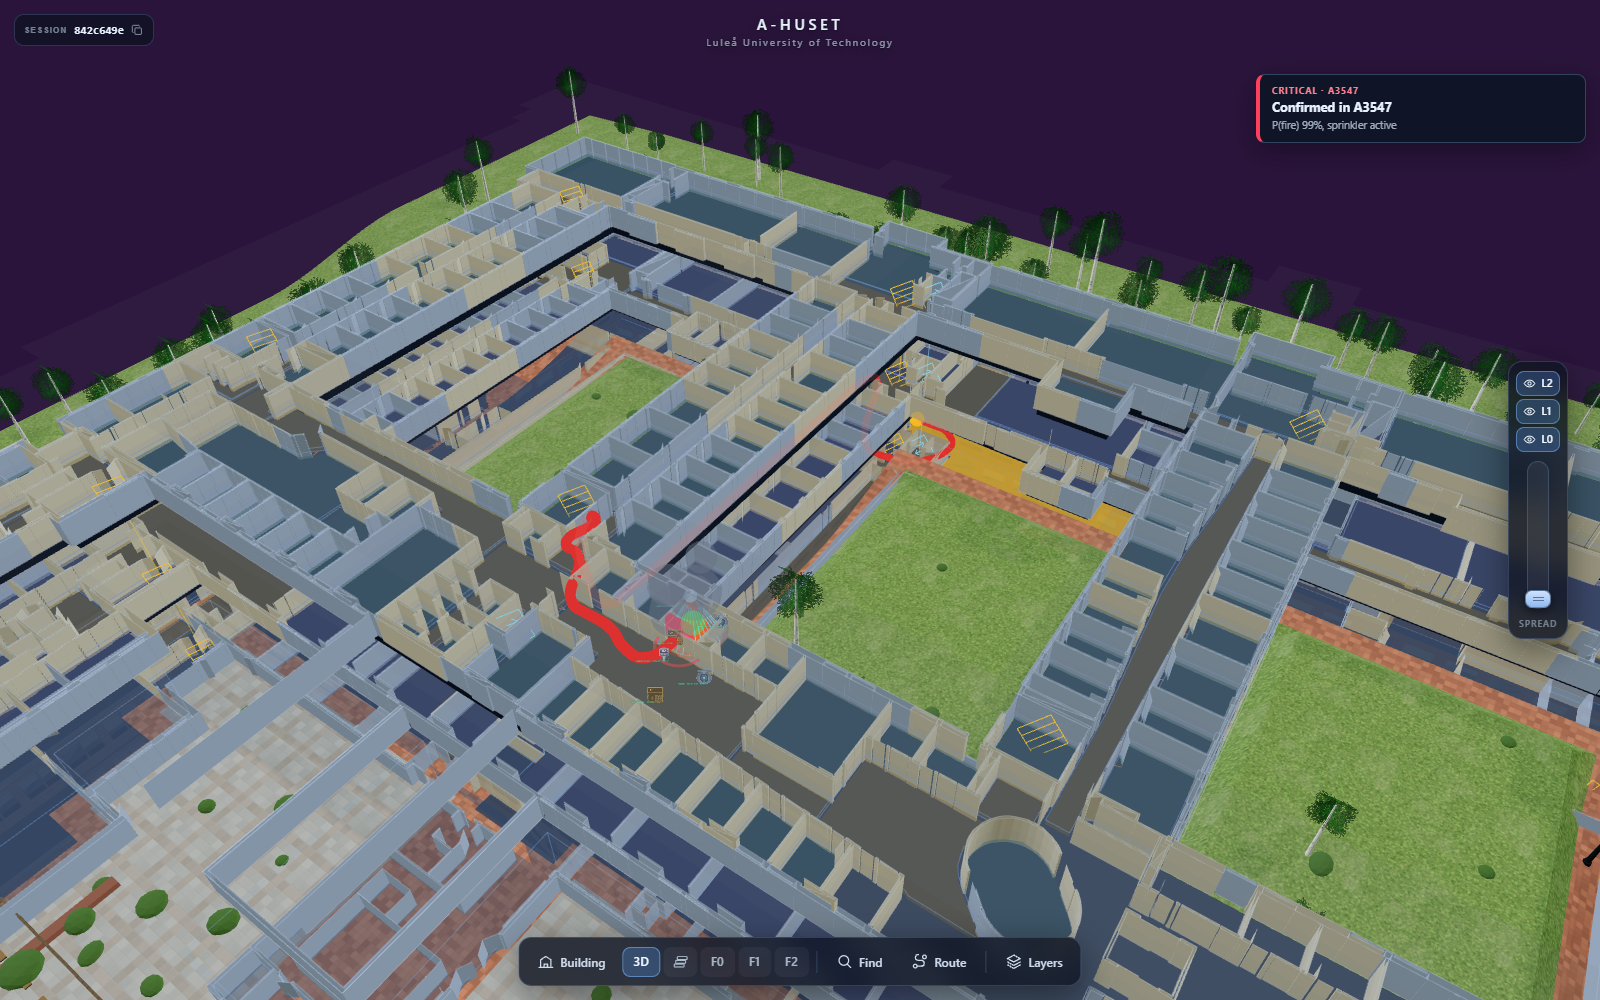
\includegraphics[width=0.49\linewidth]{images/viewer_route.png}\hfill
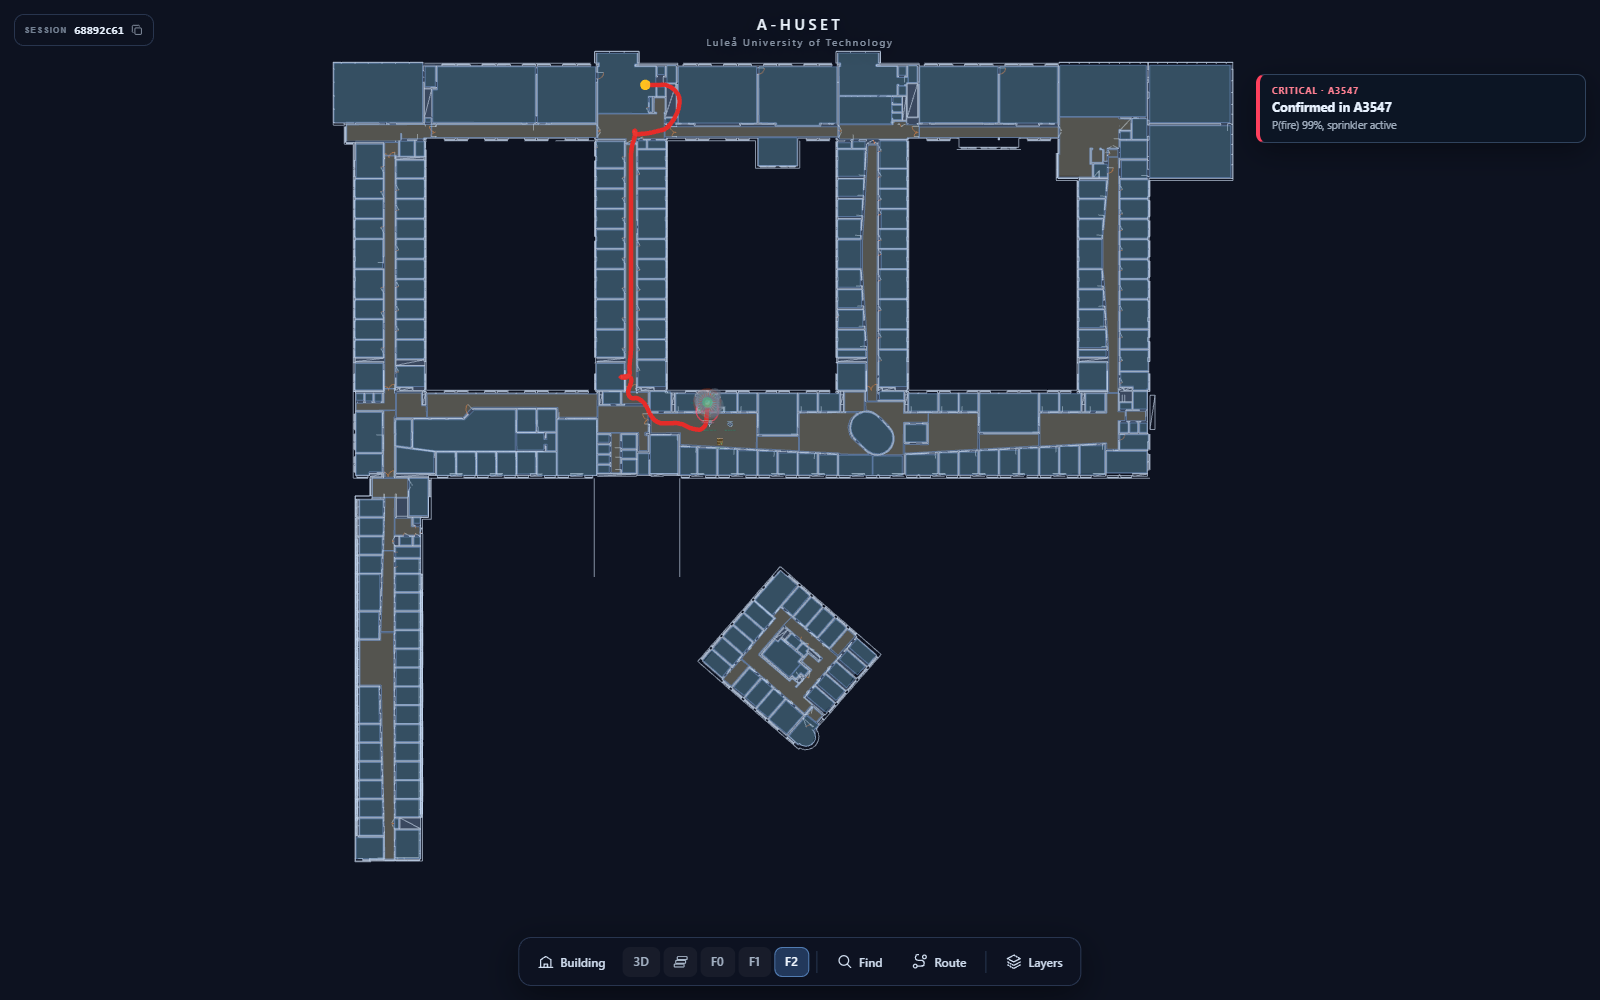
\includegraphics[width=0.49\linewidth]{images/viewer_plan.png}
\caption{The BuildSim viewer with firelab's overlays. Left: the 3D view, with the fire in the top-floor office and the escape route going down the stairwell. Right: the same route on the floor-2 plan, from the burning room to the exit.}
\label{fig:viewer}
\end{figure}

The most useful part of the panel is the least visual. The Rooms table puts the
true value of each sensor type next to what its sensor reported. The room detail
draws both on one chart. A maxed-out heat detector, a stuck smoke detector or a
drifting one shows up as a gap between two lines. The operator of a real building
never gets to see this, and it is what this project is about. Next to it, the
``Why'' bars split the probability into its parts. So 99\,\% is not a claim but a
sum. With the model installed, the same bars show what the model said it weighed,
with its answer as the top bar. The heading names which detector is speaking. The
P(fire) trace in Figure~\ref{fig:dashboard} shows the model's first answer
pulling the room back to normal before its second answer lifted it. A number on
its own would hide that. The journal below records every state change and every
command with its reason. It also records every refusal with the safety rule's
reason, and every hand-over between the model and the rule. The scorecard grades
the run as it happens: catches, misses, false alarms, the alarm delay and the RSET.
You choose the detector in the settings panel, and you can change it mid-fire. The
speed dial then shows the cap the model sets. Everything on the panel arrives over
the event stream, one snapshot per tick. The whole record can be saved as a
labelled CSV.

\section{Risks and critical reflection}\label{sec:risks}

The system does what the requirements ask. But the evaluation found five things
that deserve more doubt than a tick mark gives them.

\textbf{The dead-detector blind spot is real.} A room with two of its three sensor
types working stalled three thousandths below the confirm threshold. Its neighbour
rescued it. That is a good outcome in this building, where offices share doorways
with corridors. But it depends on the building's layout, not on the detector. The
coverage penalty should be softened, or a confirmed neighbour should be allowed to
confirm the room. Both are one-line changes. Choosing between them needs more than
one run.

\textbf{The margins are thinner than the zeros suggest.} No false alarm went off,
but cooking reached 0.749 against a threshold of 0.75. The waiting times are what
really kept it quiet. A different kitchen, a bigger pan or a slightly different
noise draw would push the probability over. The real question is whether it would
then hold for 45 seconds. I did not measure that across enough seeds to say. The
false-alarm rate here is zero in the runs I did, not zero in general.

\textbf{Containment is modelled too kindly to the neighbours and too harshly to
the fire room.} Closing the doors halved the smoke next door, which is right. It
also raised the fire room from 309 to 648\,°C. That comes from the model: water
only reduces the heat the fire releases, and a sealed room cannot run out of
oxygen. In a zone model, the sprinkler would cool the hot gas layer and the fire
would starve. The relative comparisons in Section~\ref{sec:evaluation} stand, but the absolute
temperatures should not be quoted. The 35\,°C bar in the sprinkler safety rule is
also low, and the smoulder passed it in 18\,s. A rate-of-rise condition, which
checks how fast the temperature climbs, would be easier to defend.

\textbf{One process is the right call for a simulator and the wrong one for a
building.} My proposal planned nine containers, and this report has two: the
control panel and one backend service that holds all four zones. The
reason, one simulated clock, is genuine, and the layering test keeps the zones
separable. But nothing here shows fault isolation. A fire safety system that dies
with its physics engine would not be certified. The way to split it is known and
narrow. The sensing zone already sends readings per device. The actuation zone
already takes commands with reasons. Those are the two topics a broker would
carry, and simulated time would travel as a field in every message. The
evacuation model is optimistic in the same direction. Getting 130 people out in
111\,s is a walking-speed number. It has no queues at doors and no one who
hesitates.

\textbf{The language model is the slowest part of the system, and it added the
least.} In E7 it caught the same fires as the rule, one of them 30\,s later, and
it slowed the whole simulation down to a few times real time. It also runs on a
big remote server, which is an odd fit for a project about intelligence at the
edge, and its results change from run to run. The way I connected it is sound: it
only sees sensor readings, its answer goes through the same waiting times and
safety rules, and the rule covers any room it has not answered for. The weak part
is the job I gave it. Scoring every room, again and again, is better done by a
small trained model. The language model was most useful elsewhere: in the room
with the dead smoke detector, where it trusted the other two sensors, and in the
journal, where it explains itself in words. Next time I would only ask it when the
rule is unsure or the sensors disagree. That keeps the useful part and drops most
of the cost.

\begin{longtable}[]{@{}
  >{\raggedright\arraybackslash}p{(\columnwidth - 4\tabcolsep) * \real{0.34}}
  !{\colsep}>{\raggedright\arraybackslash}p{(\columnwidth - 4\tabcolsep) * \real{0.26}}
  !{\colsep}>{\raggedright\arraybackslash}p{(\columnwidth - 4\tabcolsep) * \real{0.40}}@{}}
\toprule
\rowcolor{tablehead}
\textbf{Risk / assumption} & \textbf{Impact} & \textbf{Mitigation / decision} \\
\midrule
\endhead
Coverage penalty caps a room with two sensor types below confirm & A fire with a dead smoke detector is caught only through its neighbour & Soften the floor of the coverage factor, or let a confirmed neighbour confirm the room. Measure over many seeds \\
\rowline
Cooking probability within 0.001 of the threshold & A false alarm under a different noise draw & Waiting times hold. Add a multi-seed false-alarm rate to the harness before tuning \\
\rowline
Lumped physics with no oxygen limit and no direct cooling & Sealed fire rooms overheat. Absolute temperatures make the response look better or worse than it is & Compare results with each other, not as absolute values. A two-layer zone model is the next physics step \\
\rowline
Heat check at 35\,°C & Water released on a warm smoulder or a hot day & Require a rate of temperature rise as well as a level \\
\rowline
Single process, no fault isolation & A crash in one zone stops detection & Fine on the laptop. The zone seams become the broker topics when it is split \\
\rowline
Evacuation without queues or hesitation & RSET is a lower bound & Report it as one. Add door capacity and a pre-movement delay per role \\
\rowline
Hand-tuned detector weights & May not carry over to other buildings or sensor mixes & The CSV export and the Detector protocol are ready for a trained replacement. The rule is its baseline \\
\rowline
Language model as the per-room detector & The simulation runs only 1.4--3$\times$ real time. One alarm came 30\,s later. Results change between runs & The rule, the waiting times and the safety rules limit the harm. Only ask the model when the rule is unsure \\
\rowline
Route drawn in one viewer tab, sent once & A second tab, or a reload at the wrong moment, sees no line & Re-sending on session change is done. A replay per tab on connect would finish it \\
\bottomrule
\end{longtable}

If I had two more weeks, I would spend them on three things, in this order. First,
a multi-seed false-alarm rate. Second, the coverage fix, with that rate as its
test. Third, the trained detector my proposal promised. I would judge it against
the rule on the same recorded runs, and on whether its ``Why'' can be drawn as
bars. The system as it stands is small, explainable and measured. Its weak points
are written down here rather than found during the demo.



% ============================= References ============================
%\newpage
% No citations in the proposal; re-enable when references are added.
%\printbibliography
%\addcontentsline{toc}{section}{References}

\end{document}
